\documentclass[11pt,a4paper]{article}
\usepackage[a4paper,margin=2.6cm]{geometry}
\usepackage{iftex}
\ifPDFTeX
  \usepackage[T2A]{fontenc}
  \usepackage[utf8]{inputenc}
  \usepackage[english,russian]{babel}
\else
  \usepackage{fontspec}
  \usepackage{polyglossia}
  \setdefaultlanguage{russian}
  \setotherlanguage{english}
  \defaultfontfeatures{Ligatures=TeX}
  % Font chain: local Times New Roman -> Liberation (Overleaf) -> CMU.
  \IfFontExistsTF{Times New Roman}{%
    \setmainfont{Times New Roman}%
    \setsansfont{Arial}%
    \setmonofont{Courier New}%
    \newfontfamily\cyrillicfont{Times New Roman}%
    \newfontfamily\cyrillicfontsf{Arial}%
    \newfontfamily\cyrillicfonttt{Courier New}%
  }{%
    \IfFontExistsTF{Liberation Serif}{%
      \setmainfont{Liberation Serif}%
      \setsansfont{Liberation Sans}%
      \setmonofont{Liberation Mono}%
      \newfontfamily\cyrillicfont{Liberation Serif}%
      \newfontfamily\cyrillicfontsf{Liberation Sans}%
      \newfontfamily\cyrillicfonttt{Liberation Mono}%
    }{%
      \setmainfont{CMU Serif}%
      \setsansfont{CMU Sans Serif}%
      \setmonofont{CMU Typewriter Text}%
      \newfontfamily\cyrillicfont{CMU Serif}%
      \newfontfamily\cyrillicfontsf{CMU Sans Serif}%
      \newfontfamily\cyrillicfonttt{CMU Typewriter Text}%
    }%
  }
\fi
\usepackage{microtype}
\usepackage{mathtools,amssymb}
\usepackage{graphicx}
\usepackage{booktabs}
\usepackage{float}
\usepackage{caption}
\captionsetup{font=small,labelfont=bf}
\usepackage{enumitem}
\setlist{nosep,leftmargin=1.5em}
\usepackage{csquotes}
\usepackage[backend=biber,style=gost-numeric,sorting=none]{biblatex}
\addbibresource{references_v2.bib}
\usepackage[unicode,hidelinks]{hyperref}
\setlength{\emergencystretch}{2em}

\title{{\normalsize\normalfont\hspace*{-\leftskip}\parbox{\linewidth}{\raggedright УДК~551.513}}\\[1.5em]
Географическая дифференциация сопряжённости иерархических уровней\\
атмосферной циркуляции: атрибуция и планетарная карта}
\author{Н.~Сотириади\thanks{%
  \textbf{[ЗАПОЛНИТЬ ПЕРЕД ПОДАЧЕЙ]} организация, почтовый адрес с индексом, страна.\\
  E-mail: \texttt{n.sotiriadi@gmail.com}. ORCID: \textbf{[ЗАПОЛНИТЬ]}.}}
\date{2026}

\begin{document}
\maketitle

\begin{abstract}
В первой статье серии показано, что сопряжённость соседних масштабных уровней --- мера того, насколько размещение мезомасштабной изменчивости предопределено соседним крупным уровнем, --- является устойчивым региональным инвариантом нижнетропосферной циркуляции. Настоящая работа отвечает на следующий, собственно географический вопрос: чем определяется географическая дифференциация этого инварианта. Единицей анализа вместо 39 региональных областей служит ячейка мозаичной карты (реанализ ERA5, относительный вихрь на изобарической поверхности 850~гПа): 144 ячейки внутри двенадцати равновеликих областей и глобальная сетка из 936 ячеек ($60^\circ$~ю.\,ш.\,--\,$60^\circ$~с.\,ш., два сезона 2023~г.). Проверяются три конкурирующих объяснения географии карты: экзогенные граничные условия, состояние циркуляции и артефакт наблюдательной системы. Карта предсказуема по внешним ковариатам ($R^2=0{,}40$--$0{,}54$ при выбывании целых регионов и секторов долготы, $p=0{,}001$) и эффективно одномерна: одна синоптическая вихревая активность внетропических штормовых путей даёт 85\,\% полного качества предсказания. Связь двухканальна: высокая штормовая активность сопровождается повышением сопряжённости через дисперсионную структуру, отражаемую спектром, высокая конвективная неустойчивость --- её понижением сверх спектра; контрольная мишень (наклон спектра) предсказывается не хуже, но другим набором ковариат. Свободный модельный расчёт без усвоения наблюдений воспроизводит карту на 97\,\% достижимого согласия: гипотеза об артефакте отвергнута. Экзогенные условия сами по себе дают 90\,\% качества предсказания, поэтому итоговая формулировка объединяет оба яруса: географическая дифференциация сопряжённости структурирована через размещение циркуляционных режимов в географическом пространстве. При потолке надёжности карты $R^2=0{,}914$ заявленные ковариаты объясняют 59\,\% воспроизводимой дисперсии; остаток воспроизводим и не сводится к спектру. Тропический избыток межгодовой изменчивости связан с Междекадным тихоокеанским колебанием, а гипотеза статичности инварианта подтверждена прямой проверкой. Работа устанавливает атрибуцию, а не механизм.

\smallskip
\noindent\textbf{Ключевые слова:} региональная география, физико-географическое районирование, сопряжённость масштабов, атмосферная циркуляция, атрибуция, штормовые пути, конвективный режим, реанализ, свободный модельный расчёт.
\end{abstract}

\begin{english}
\begin{abstract}
\noindent\textbf{Geographical differentiation of the coupling between hierarchical levels of the
atmospheric circulation: attribution and a planetary map}

\smallskip\noindent N.~Sotiriadi

\smallskip\noindent The first paper of this series established that the coupling of neighbouring
scale levels --- a measure of how far the placement of mesoscale variability is set by the adjacent
large level --- is a stable regional invariant of the lower-tropospheric circulation. The present
paper asks what governs the geographical differentiation of that invariant. The unit of analysis is
a mosaic tile rather than a region (ERA5 reanalysis, relative vorticity at 850~hPa): 144 tiles inside
twelve equal-area boxes, and a global grid of 936 tiles ($60^\circ$S--$60^\circ$N, two seasons of
2023). Three competing explanations of the map are tested: exogenous boundary conditions, the state
of the circulation, and an artefact of the observing system. The map is predictable from external
covariates ($R^2=0.40$--$0.54$ under leave-one-region-out and leave-one-longitude-sector-out,
$p=0.001$) and effectively one-dimensional: synoptic eddy activity alone delivers 85\,\% of the full
predictive skill. The association is two-channel: storm-track activity goes with higher coupling
through the same variance structure the spectrum sees, whereas convective instability goes with lower
coupling beyond the spectrum; the control target (spectral slope) is predicted equally well but by a
disjoint set of covariates. A free-running model integration that assimilates no observations
reproduces the map at 97\,\% of the attainable agreement, so the artefact hypothesis is rejected.
Exogenous conditions alone recover 90\,\% of the predictive skill; the geographical differentiation
of coupling is therefore structured through the placement of circulation regimes in geographical
space. Against a map reliability ceiling of $R^2=0.914$ the declared covariates explain 59\,\% of
the reproducible variance; the residual is reproducible and is not reducible to the spectrum. The
paper establishes attribution, not mechanism.

\smallskip
\noindent\textbf{Keywords:} regional geography, physical-geographical regionalisation, scale
coupling, atmospheric circulation, attribution, storm tracks, convective regime, reanalysis,
free-running model integration.
\end{abstract}
\end{english}

\section{Введение}
\label{sec:intro}

\subsection{От регионального инварианта к вопросу об атрибуции}

Региональная дифференциация атмосферной циркуляции традиционно описывается климатологией её ведущих организаторов: внетропических штормовых путей --- полос повышенной повторяемости и интенсивности циклонических возмущений умеренных широт \cite{HoskinsValdes1990,Chang2002,HoskinsHodges2005,Shaw2016} --- и режимов глубокой конвекции \cite{Houze2004,Feng2021}. В первой статье серии\footnote{Сотириади~Н. Сопряжённость иерархических уровней атмосферной циркуляции как региональный инвариант (первая статья настоящей серии; подана в печать). Протоколы, код и численные результаты обеих работ открыты в едином репозитории: \url{https://github.com/Theclimateguy/Shroedinger}.} к этому описанию добавлена характеристика иного типа: по полю относительного вихря на поверхности 850~гПа построен профиль сопряжённости соседних октавных уровней~$P$ --- мера того, насколько размещение мезомасштабной изменчивости предопределено соседним крупным уровнем, --- и показано, что эта величина удовлетворяет операциональному определению инварианта динамики геосистем \cite{Puzachenko1986,Puzachenko2004,Puzachenko2010} в традиции выделения уровней организации регионального климата \cite{Krenke2019}: она устойчива к смене сезона, года, фазы Эль-Ниньо~--- Южного колебания (ЭНСО), источника данных (MERRA-2 \cite{Gelaro2017}) и схемы разбиения территории, содержит воспроизводимую информацию сверх спектра поля и воспроизводится в модельном расчёте, не усваивающем наблюдений. Обоснование самой конструкции, полное операциональное описание процедуры оценивания и каталог проверенных и отвергнутых интерпретаций даны там же и здесь не повторяются.

Настоящая работа ставит следующий, собственно географический вопрос: \emph{чем определяется географическая дифференциация инварианта} --- в каких отношениях его карта находится с известными организаторами циркуляции и с экзогенными граничными условиями (орография, конфигурация суши и океана, температура поверхности океана). Рабочая рамка вопроса --- цепочка <<географическая конфигурация $\to$ организация атмосферных процессов $\to$ сопряжённость уровней>>: экзогенная конфигурация задаёт, где складываются организующие процессы --- штормовые пути и конвективные режимы, --- а их организация проявляется в устройстве межуровневых связей. Задача атрибуции --- проверить эту цепочку статистически, различая её звенья по причинному статусу. Ответ одновременно проверяет содержательность величины --- атрибутируема ли она физическим условиям --- и открывает путь к её прикладному использованию: характеристика, предсказуемая по условиям и картируемая глобально, может служить координатой районирования территорий по устройству межуровневых связей.

Слово <<географический>> употребляется далее в трёх различимых смыслах, и работа разделяет их с самого начала. Первый --- \emph{географическое положение} (широта, долгота); второй --- \emph{физико-географические свойства территории} (высота и расчленённость рельефа, соотношение суши и моря, изрезанность берега, температура поверхности океана); третий --- \emph{тип циркуляционного режима над территорией} (активность штормовых путей, конвективный режим). Первые два смысла отсылают к условиям, экзогенным по отношению к циркуляции; третий --- к состоянию, складывающемуся вместе с ней. Соответственно проверяемое здесь утверждение --- не <<география определяет сопряжённость уровней>>, а более точное: \emph{географическая дифференциация сопряжённости структурирована через размещение атмосферных циркуляционных режимов в географическом пространстве}, причём само это размещение задано экзогенной конфигурацией. Такая постановка продолжает отечественную традицию выделения уровней организации геосистем и физико-географического районирования \cite{Sochava1978,Isachenko1991,Bertrand1968} и примыкает к общему для наук о Земле вопросу о масштабе, на котором территория обладает собственной организацией \cite{Simon1962,Levin1992,WuLoucks1995}.

Здесь же уместна терминологическая оговорка, определяющая всё дальнейшее чтение. Эмпирически величина~$P$ измеряет \emph{пространственную со-организацию} активности соседних масштабных уровней --- то, насколько согласованно они размещены по территории. Слово <<сопряжённость>> служит кратким именем этого факта и не подразумевает ни динамической связи между масштабами, ни переноса энергии: обе интерпретации прямо проверены и отвергнуты в первой статье серии. Высокое~$P$ читается как признак географического режима, в котором активность соседних масштабов сильно пространственно организована, --- не как доказательство <<сильного взаимодействия>> масштабов. Соответственно везде, где ниже говорится о <<канале>> или о том, что тот или иной режим <<повышает>> либо <<понижает>> сопряжённость, имеется в виду устойчивая статистическая связь заданного знака, а не установленный физический процесс.

Первая попытка атрибуции была предпринята на региональной выборке и закончилась поучительной неудачей: на двенадцати региональных скалярах пять средовых ковариат (модуль широты, сдвиг ветра, климатология конвективной неустойчивости, доля суши, орография) дали при перекрёстной проверке с исключением по одному отрицательную объяснённую дисперсию ($R^2_{\mathrm{LOO}}=-0{,}62$, $p=0{,}65$). Урок здесь методический: двенадцать точек не способны корректно вместить ни одно семейство ковариат, и содержательные выводы на такой выборке неотличимы от подгонки. Решение --- смена единицы выборки: переход от региональных скаляров к мозаичной карте, где единицей выступает ячейка мозаики (далее --- тайл) размером в сотни километров, а региональная принадлежность тайлов используется как блокирующий фактор статистики. Число степеней свободы при этом растёт на порядок ($n\approx144$, затем $n\approx936$), а межрегиональные смешения контролируются схемой выбывания целых регионов или секторов долготы.

Задачи работы: (1)~построить тайловую, а затем глобальную карту тонкомасштабного~$P$ с суррогатной поправкой и проверить её согласованность с региональным уровнем первой статьи; (2)~выполнить статистически корректную атрибуцию географии карты по заранее заявленным внешним ковариатам, с отрицательным контролем и контрольной мишенью; (3)~проверить природу карты сопоставлением со свободным модельным расчётом; (4)~атрибутировать ранее обнаруженный тропический избыток межгодовой изменчивости по заранее названным климатическим индексам; (5)~проверить прямое следствие статуса инварианта --- гипотезу статичности (разд.~\ref{sec:static}).

\subsection{Три конкурирующие гипотезы}
\label{sec:hypotheses}

Вопрос о географии карты~$P$ распадается на выбор между тремя объяснениями, каждое из которых имеет собственное проверяемое следствие. Гипотезы и распределение ковариат по ярусам зафиксированы протоколом до вычислений.

\emph{H1, экзогенная.} География~$P$ определяется стационарными граничными условиями территории --- рельефом, конфигурацией суши и океана, широтой, полем температуры поверхности океана. Следствие: карта предсказуема по одному ярусу~1, а характеристики циркуляционного режима не добавляют к предсказанию существенного.

\emph{H2, циркуляционная.} География~$P$ определяется состоянием циркуляции --- активностью внетропических штормовых путей и конвективным режимом. Следствие: ведущие нагрузки принадлежат ярусу~2, и связь сохраняется \emph{внутри} климатически однородных областей, где экзогенные условия почти постоянны.

\emph{H3, артефактная.} Карта~$P$ --- свойство наблюдательной сети и системы усвоения, а не атмосферы. Следствие: карта не должна воспроизводиться расчётом, не усваивающим атмосферных наблюдений.

Существенно, что H1 и H2 не исключают друг друга. Если экзогенная конфигурация задаёт, \emph{где} располагаются циркуляционные режимы, то оба яруса будут читать одну и ту же карту, и содержательным результатом окажется не победа одного объяснения над другим, а мера их совместности. Именно поэтому проверка построена так, чтобы измерить вклад каждого яруса по отдельности, а не выбрать между ними голосованием: разделение ковариат по ярусам, корреляции внутри регионов, нуль-модель, сохраняющая всю зональную структуру, и сопоставление со свободным модельным расчётом. Ответы даны в разд.~\ref{sec:armA}--\ref{sec:model} и сведены в разд.~\ref{sec:interp}.

\subsection{Гипотеза статичности}

Величина~$P$ заявлена в первой статье как \emph{статичный} инвариант сложившегося циркуляционного режима: характеристика архитектуры уже установившейся организации, а не переменная, несущая собственную динамику. Из этого статуса вытекает прямое и проверяемое следствие: при перестройке режима такая величина не должна опережать перестройку и не должна превосходить по чувствительности стандартные показатели среднего поля. Это следствие --- не дополнительное ограничение, навешиваемое на результат, а необходимое свойство инварианта, подлежащее проверке наравне с остальными; этой проверке посвящён разд.~\ref{sec:static}.

Работа сознательно остаётся в рамках эмпирической атрибуции и картирования. Интерпретирующая рамка --- язык квазинеизменных полей ограничений и функционалов инвариантной меры --- вынесена в завершающую, третью статью серии; здесь она затрагивается лишь в объёме одного раздела (разд.~\ref{sec:interp}).

\section{Материалы и методы}
\label{sec:data}

\subsection{Данные и две части протокола}

Материал обеих частей --- реанализ ERA5 \cite{Hersbach2020,Soci2024}: составляющие ветра на изобарической поверхности 850~гПа, сетка $0{,}25^\circ$, шаг 6~ч, поле относительного вихря --- идентично первой статье серии. Обе части выполнены по единому протоколу, зафиксированному до вычислений (все критерии, пороги и нуль-модели заданы заранее; отступления фиксировались в журнале протокола).

\emph{Часть~A} --- 144 тайла внутри двенадцати равновеликих областей первой статьи (12 областей $\times$ 12 тайлов): сетка $3\times4$ на область, ячейки $\approx667\times700$~км. Использованы только те поля, что уже имелись в архиве программы исследования (сезонные окна 2021--2024~гг.).

\emph{Часть~B} --- глобальная сетка из 936 тайлов: широтные полосы по $6^\circ$ ($\approx$667~км), долготные ячейки по 700~км на центральной широте полосы (точное кольцевое покрытие без остатка), пояс $60^\circ$~ю.\,ш.\,--\,$60^\circ$~с.\,ш.; два независимых сезона --- январь--март и июль--сентябрь 2023~г. Из анализа исключены 34 тайла со средней высотой рельефа более 1200~м (поверхность 850~гПа ниже подстилающей); в атрибуции участвуют 902 тайла.

\emph{Целевая величина} --- тонкомасштабный профиль~$P$ с суррогатной поправкой: сопряжённость огибающих в диапазоне полос 50--400~км, вычисленная по внутренней маске тайла и взятая в превышении над медианой 99 фазовых суррогатов, генерируемых отдельно для каждой пары <<тайл--окно>>. Методика идентична первой статье и здесь не пересказывается.

Полосы 50--400~км частично или полностью лежат ниже эффективного разрешения реанализа: правило 4--7 шагов сетки даёт для ERA5 около 125--220~км \cite{Skamarock2004}, прямая спектральная оценка --- 500--600~км в средних широтах и порядка 1000~км в тропиках \cite{Bolgiani2022}. Работа с тонкими полосами тем не менее корректна по трём причинам. Суррогатная поправка сравнивает наблюдаемое поле с полем той же спектральной структуры, прошедшим тот же вычислительный тракт, --- вклад численной диссипации и параметризаций одинаков в измеряемой величине и в вычитаемом фоне. Карта воспроизводится свободным расчётом другой конфигурации модели на общей сетке $0{,}5^\circ$ на 97\,\% достижимого согласия (разд.~\ref{sec:model}) --- тонкополосная структура не является артефактом конкретного тракта усвоения. Наконец, мозаичная карта согласована с региональным уровнем первой статьи ($\rho=0{,}874$), где эффект выдерживает контроль, ограниченный заведомо разрешёнными масштабными ступенями. Остающееся ограничение обсуждается в разд.~\ref{sec:limitations}.

\subsection{Ковариаты и их причинный статус}

Внешние ковариаты разбиты на два яруса, и граница между ними задана протоколом \emph{до} вычислений --- она определяет допустимый язык интерпретации, а не подбирается под результат.

\emph{Ярус~1 --- экзогенные граничные условия} (допустим направленный язык <<формируют>>): средняя высота рельефа в тайле и его расчленённость (стандартное отклонение высоты); доля суши; контрастность подстилающей поверхности суша--море (стандартное отклонение маски суши внутри тайла --- мера изрезанности берега, максимальная при равном соотношении суши и моря); модуль широты; средний модуль градиента температуры поверхности океана (ТПО).

\emph{Ярус~2 --- совместно складывающиеся характеристики состояния} (только язык совместной организации, без направленности): климатология конвективной доступной потенциальной энергии CAPE за 2021--2024~гг. \cite{RiemannCampe2009} --- показатель конвективного режима территории --- и синоптическая кинетическая энергия вихрей (дисперсия ветра относительно скользящего 5-суточного среднего) --- стандартная мера активности внетропических штормовых путей, восходящая к классическим полосовым климатологиям синоптической изменчивости \cite{Blackmon1976,HoskinsHodges2005,HoskinsHodges2019}.

\emph{Отрицательный контроль} --- индекс листовой поверхности (климатология ERA5, сумма компонент низкой и высокой растительности): биологический показатель, механистически неправдоподобный как фактор сопряжённости масштабов 50--400~км на уровне 850~гПа. Ожидаемый исход --- отсутствие прироста предсказания; значимый прирост означал бы скрытое смешение в схеме, а не открытие.

\subsection{Статистический дизайн}

\emph{Нуль-модели атрибуции.} В части~A нулевое распределение строится перестановками региональных меток целыми блоками тайлов (999 повторов): тайлы одного региона всегда перемещаются вместе, поэтому внутрирегиональная зависимость сохраняется в нуле. В части~B нуль --- циклический поворот долготной сетки ковариат относительно карты~$P$ на случайный сдвиг не менее $30^\circ$ (999 повторов). Поворот сохраняет полную пространственную автокорреляцию обоих полей и, поскольку модуль широты инвариантен относительно поворота долготы, сохраняет и всю зональную структуру целиком: значимость теста удостоверяет именно \emph{незональную}, долготную часть атрибуции --- привязку карты к фактическому положению штормовых путей и конвективных очагов, а не только к широтному градиенту.

\emph{Проверка предсказания и эффективная размерность.} Предсказание проверяется выбыванием целыми блоками --- по региону (часть~A) либо по одному из шести секторов долготы по $60^\circ$ (часть~B); сообщаемое $R^2$ всегда относится к предсказанию на не участвовавших в подгонке блоках. Эффективная размерность оценивается прямым пошаговым отбором ковариат с тем же блочным выбыванием; $k_{80}$ --- число ковариат, достаточное для 80\,\% полного качества.

\emph{Потолок надёжности карты} --- внутрисезонное расщепление выборки пополам: сроки каждой пары <<тайл--сезон>> делятся по чётности на две непересекающиеся половины, каждая половина привязывается к собственным 99 суррогатам, надёжность полной выборки восстанавливается поправкой Спирмена--Брауна \cite{Spearman1910,Brown1910}. Подчеркнём выбор именно внутрисезонной оценки: межсезонная согласованность двух карт ($r=0{,}776$) занижает потолок, поскольку списывает реальное сезонное изменение карты на счёт шума.

\emph{Контрольная (плацебо) мишень} --- наклон пространственного спектра тайла: если бы атрибуция~$P$ лишь повторяла атрибуцию спектра, нагрузки двух мишеней совпадали бы.

\section{Результаты}
\label{sec:results}

\subsection{Глобальная карта сопряжённости}
\label{sec:map}

Центральный результат работы --- глобальная карта тонкомасштабного~$P$ с суррогатной поправкой (рис.~\ref{fig:global}), построенная по 902 тайлам пояса $60^\circ$~ю.\,ш.\,--\,$60^\circ$~с.\,ш. и двум сезонам 2023~г. Прежде всякой статистики её стоит прочесть как карту.

Максимумы образуют узнаваемую циркуляционную географию: сплошное кольцо над Южным океаном, северотихоокеанский и североатлантический штормовые пути --- в точности те пояса, где внетропическая бароклинная активность организует поле сразу на нескольких масштабах \cite{HoskinsValdes1990,Chang2002,HoskinsHodges2005,Shaw2016}. Минимумы столь же узнаваемы и приурочены к очагам глубокой конвекции: Амазонии, бассейну Конго и Индонезийскому архипелагу (Морскому континенту) \cite{NealeSlingo2003,Feng2021}. Промежуточные значения занимают субтропические океаны и внутриматериковые области умеренного пояса. Таким образом, первое прочтение карты --- содержательно географическое: она разделяет территории по типу господствующего циркуляционного режима.

Карта не сводится к широтной зональности. Описательное разложение её дисперсии даёт 51\,\% на широтные полосы по $6^\circ$, ещё 10\,\% на долготные секторы внутри полос и 39\,\% на изменчивость внутри ячеек $6^\circ\times60^\circ$. Почти половина рисунка незональна, и именно эта половина различает конкретные территории, а не только климатические пояса.

Карта сезонно устойчива: медиана модуля разности между картами января--марта и июля--сентября составляет 0,016 при 90-м перцентиле 0,048 (рис.~\ref{fig:seasons}). Дальнейшее изложение отвечает на четыре вопроса об этой карте: воспроизводима ли она и что даёт переход к более мелкой единице выборки (разд.~\ref{sec:armA}); чем связана её география (разд.~\ref{sec:armB}); насколько полно она объяснена и что остаётся в остатке (разд.~\ref{sec:residual}); наконец, является ли она свойством атмосферы или наблюдательной системы (разд.~\ref{sec:model}).

\begin{figure}[t]
\centering
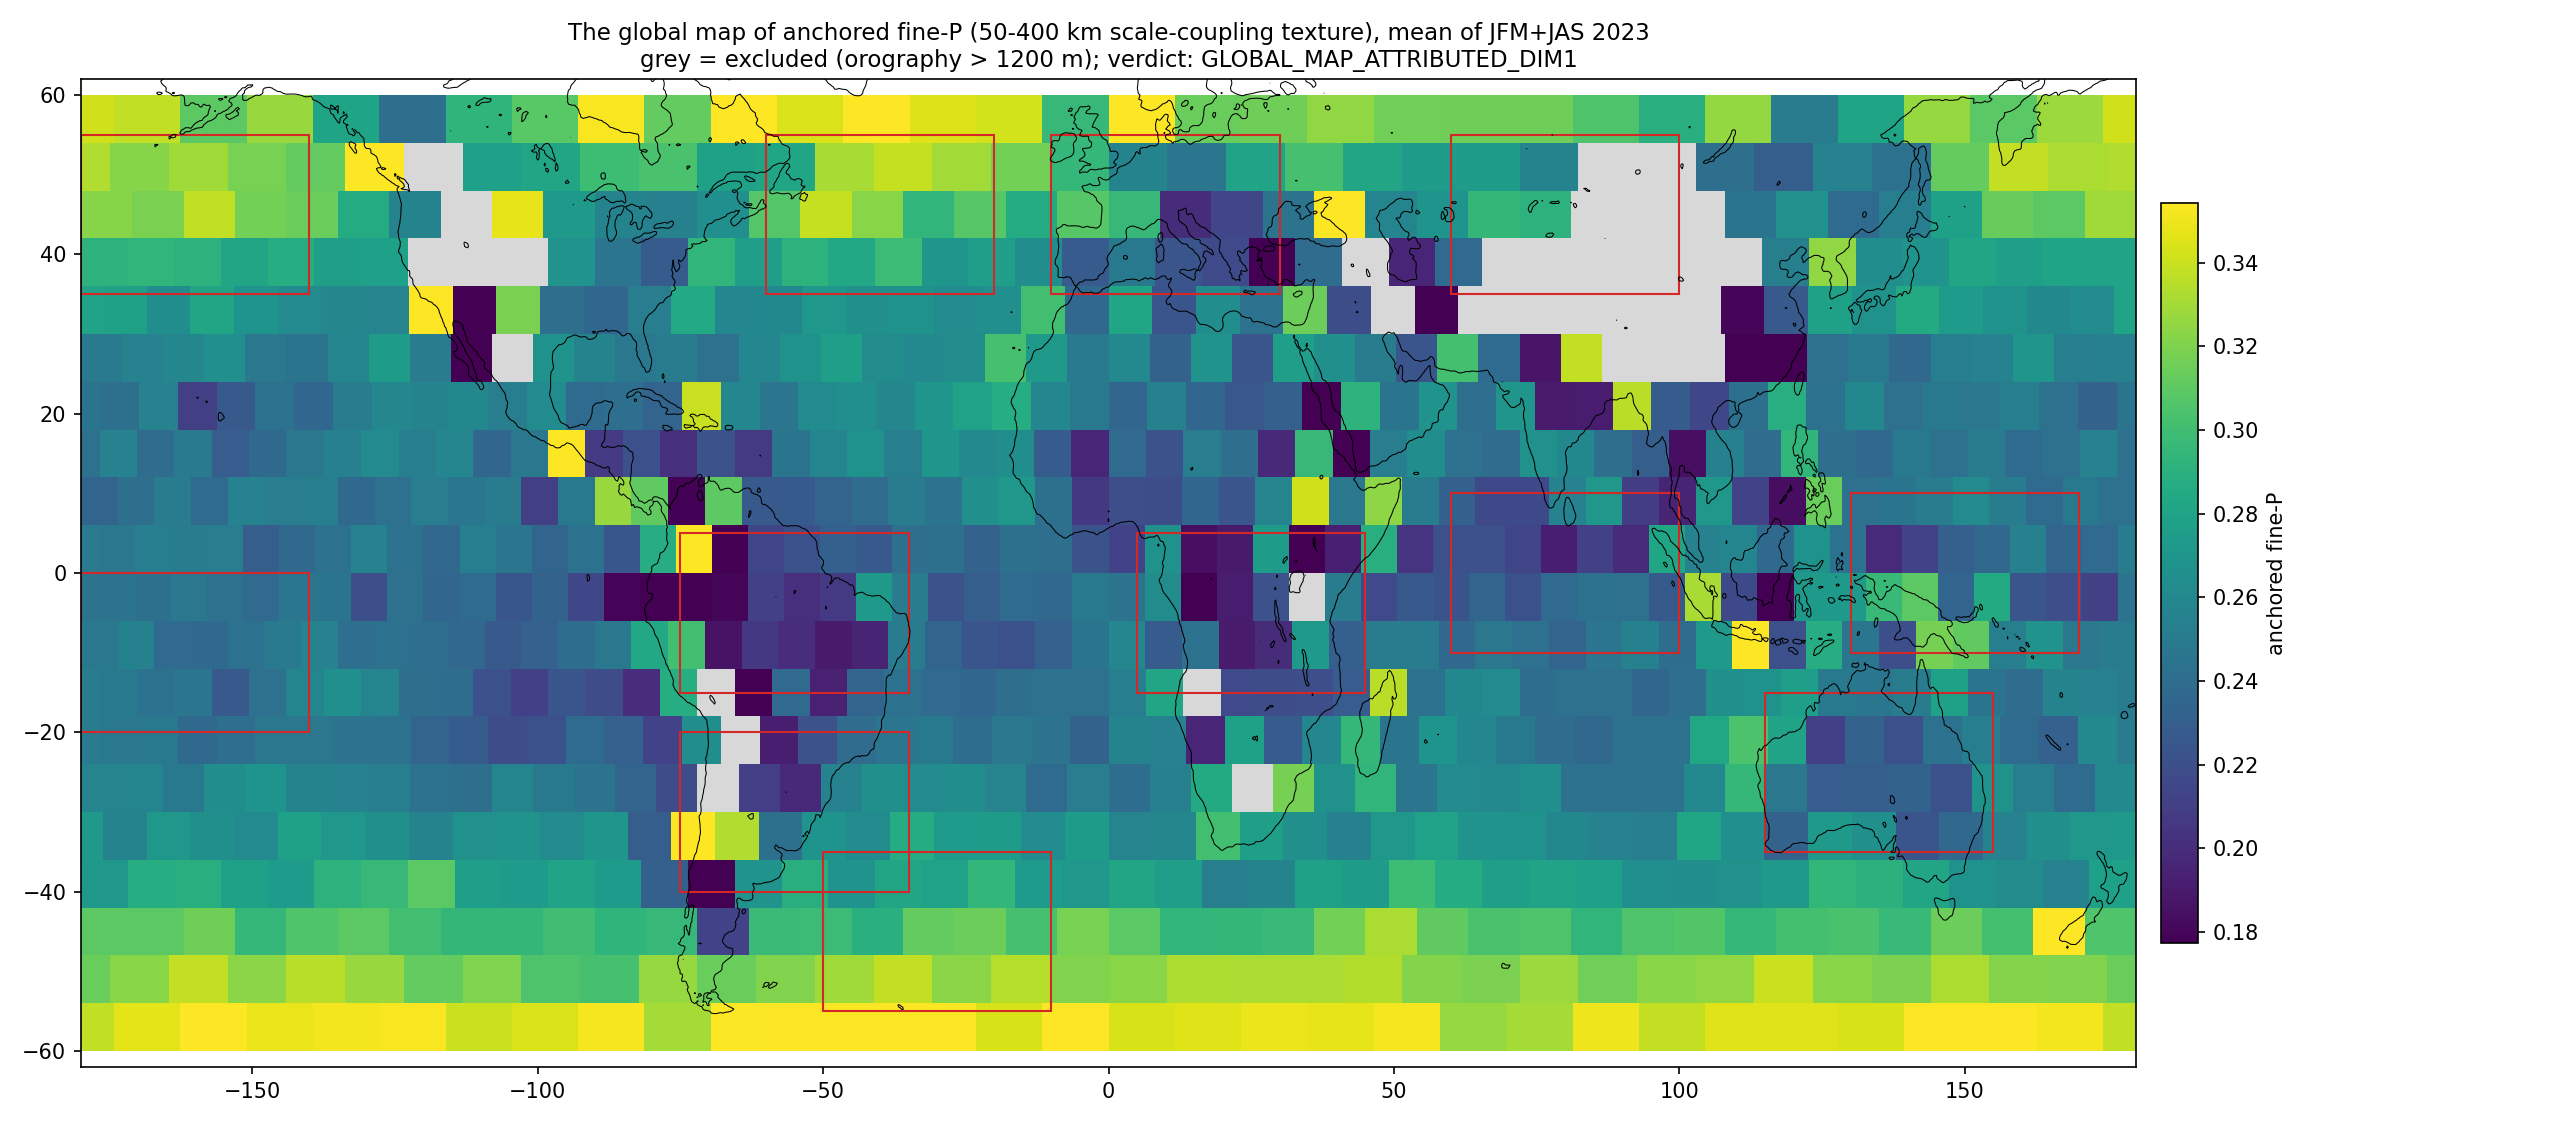
\includegraphics[width=\linewidth]{figures/fig2_global_map.png}
\caption{Глобальная карта тонкомасштабного $P$ с суррогатной поправкой (сопряжённость полос 50--400~км), среднее сезонов январь--март и июль--сентябрь 2023~г., 936 тайлов, $60^\circ$~ю.\,ш.\,--\,$60^\circ$~с.\,ш. Серым --- тайлы, исключённые по орографии (средняя высота более 1200~м); красные рамки --- двенадцать областей программы. Максимумы --- кольцо штормовых путей Южного океана, а также северотихоокеанский и североатлантический штормовые пути; минимумы --- Амазония, бассейн Конго и область муссонной конвекции Индонезийского архипелага (Морского континента).}
\label{fig:global}
\end{figure}

\subsection{Согласованность и внутрирегиональная структура (часть A)}
\label{sec:armA}

Первая проверка карты --- согласованность с региональным уровнем первой статьи. На 144 тайлах внутри двенадцати равновеликих областей ранговая корреляция тайловых значений с региональными составляет $\rho=0{,}874$ при заранее заданном пороге 0,7 (табл.~\ref{tab:armA}, рис.~\ref{fig:tiles}). Переход к более мелкой единице выборки, следовательно, не порождает новой величины, а разрешает уже установленную.

Разрешает в буквальном смысле. Описательное разложение дисперсии тайловой карты даёт 51\,\% на межрегиональную и 49\,\% на внутрирегиональную составляющую: половина географии сопряжённости живёт \emph{ниже} регионального уровня и на выборке из двенадцати чисел попросту не видна. Это и делает тайловую единицу выборки необходимой.

Атрибуция на этой выборке состоялась. В части~A информативны пять ковариат из восьми (расчленённость рельефа, доля суши, изрезанность берега, CAPE, вихревая энергия): модуль широты, градиент ТПО и средняя высота рельефа практически вырождены внутри отдельной области и работают только на глобальной сетке. Эти пять ковариат предсказывают тайловый~$P$ вне региона подгонки с $R^2=0{,}404$ при 95-м перцентиле блочного нуля $-0{,}007$.

Главный результат части~A, однако, не в величине $R^2$, а в том, что два фактора выдерживают самую жёсткую из возможных проверок --- корреляцию \emph{внутри} регионов, которую не может породить никакое межрегиональное смешение (рис.~\ref{fig:attrA}). По всей выборке 144 тайлов конвективный режим связан с сопряжённостью отрицательно ($\rho=-0{,}61$), синоптическая вихревая активность --- положительно ($\rho=+0{,}59$; оба $p=0{,}002$ при блочном нуле). Существеннее, однако, что обе связи выживают при переходе к внутрирегиональной статистике: средняя по двенадцати регионам корреляция составляет $-0{,}36$ для CAPE (отрицательна в 10 регионах из 12) и $+0{,}39$ для вихревой энергии (положительна в 11 из 12), в обоих случаях $p=0{,}001$ при перестановочном нуле внутри регионов. Это прямое эмпирическое следствие H2: связь сохраняется там, где экзогенные условия почти постоянны. Контрольная мишень показывает, что перед нами не пересказ спектра: наклон спектра тоже атрибутируем ($R^2=0{,}31$, $p=0{,}004$), но другими ковариатами: расчленённость рельефа $+0{,}82$, доля суши $+0{,}67$, изрезанность берега $+0{,}60$ --- против $+0{,}15$ у CAPE и $-0{,}23$ у вихревой энергии.

Дополнительное, описательное (апостериорное, помеченное так и в протоколе) двухслойное прочтение уточняет структуру связи. Если перед атрибуцией удалить из тайлового~$P$ часть, линейно предсказуемую по спектральным признакам самого тайла, совместная атрибуция исчезает ($R^2=-0{,}055$, $p=0{,}15$), однако отрицательная связь с CAPE выживает внутри регионов (10 из 12, средняя $\rho=-0{,}34$), а связь с вихревой энергией --- нет (8 из 12, $\rho\approx+0{,}03$). Отсюда двухканальная \emph{структура связи}: повышение сопряжённости при высокой штормовой активности проходит преимущественно через ту же дисперсионную структуру, которую видит спектр, тогда как понижение при высокой конвективной неустойчивости лежит сверх того, что видит спектр. Правдоподобное, но не проверенное в настоящей работе прочтение состоит в следующем: интермиттентная, локально порождаемая завихренность мезомасштабных конвективных систем \cite{Houze2004,Feng2021} --- процесс с выраженным пороговым характером \cite{PetersNeelin2006}, быстро порождающий собственную мезомасштабную изменчивость, слабо связанную с крупным масштабом \cite{Zhang2007,RotunnoSnyder2008,Judt2020}, --- ослабляет пространственную со-организацию соседних уровней, тогда как организованные бароклинные возмущения штормовых путей её усиливают. Подчеркнём границу: здесь установлена статистическая связь и её канальное разделение, но не механизм; проверка механизма --- предмет завершающей статьи серии.

Апостериорная проверка (не входившая в зафиксированный протокол) связывает часть~A с флагманским примером первой статьи. Модель атрибуции, обученная на десяти регионах без бассейнов Конго и Амазонии, воспроизводит внутреннюю географию их 24 отложенных тайлов (ранговая корреляция наблюдённого и предсказанного $+0{,}59$), но почти не воспроизводит межбассейновый контраст: наблюдаемая разность региональных средних $+0{,}051$, предсказанная --- лишь $+0{,}004$. Контраст двух бассейнов, установленный в первой статье, лежит, таким образом, преимущественно \emph{сверх} пяти ковариат части~A --- в той же воспроизводимой остаточной географии, что и очаги остатка глобальной карты (разд.~\ref{sec:residual}); его объяснение --- предмет завершающей статьи серии.

\begin{table}[t]
\centering
\caption{Часть A: сводка проверок на 144 тайлах внутри 12 равновеликих областей. LOO --- выбывание по региону; блочный нуль --- перестановки на уровне регионов.}
\label{tab:armA}
\small
\begin{tabular}{@{}p{0.44\linewidth}p{0.50\linewidth}@{}}
\toprule
Проверка & Итог\\
\midrule
Согласованность с региональным уровнем первой статьи & $\rho=0{,}874$ (заранее заданный порог 0,7)\\
Атрибуция, выбывание по региону & $R^2=0{,}404$; $p=0{,}001$\\
Ведущие факторы: связь по всей выборке 144 тайлов & CAPE: $\rho=-0{,}61$; вихревая энергия: $\rho=+0{,}59$ (оба $p=0{,}002$, блочный нуль); рельеф, доля суши, изрезанность берега --- незначимы\\
Те же факторы \emph{внутри} регионов (устраняет межрегиональные смешения) & CAPE: средняя по регионам $\rho=-0{,}36$, знак отрицателен в 10 из 12 регионов, $p=0{,}001$; вихревая энергия: средняя $\rho=+0{,}39$, знак положителен в 11 из 12, $p=0{,}001$ (нуль --- перестановки внутри регионов)\\
Контрольная мишень: атрибуция наклона спектра & $R^2=0{,}31$, $p=0{,}004$, но с иными нагрузками (орография $+0{,}82$, суша $+0{,}67$, CAPE и вихревая энергия $\approx0$)\\
\bottomrule
\end{tabular}
\end{table}

\begin{figure}[t]
\centering
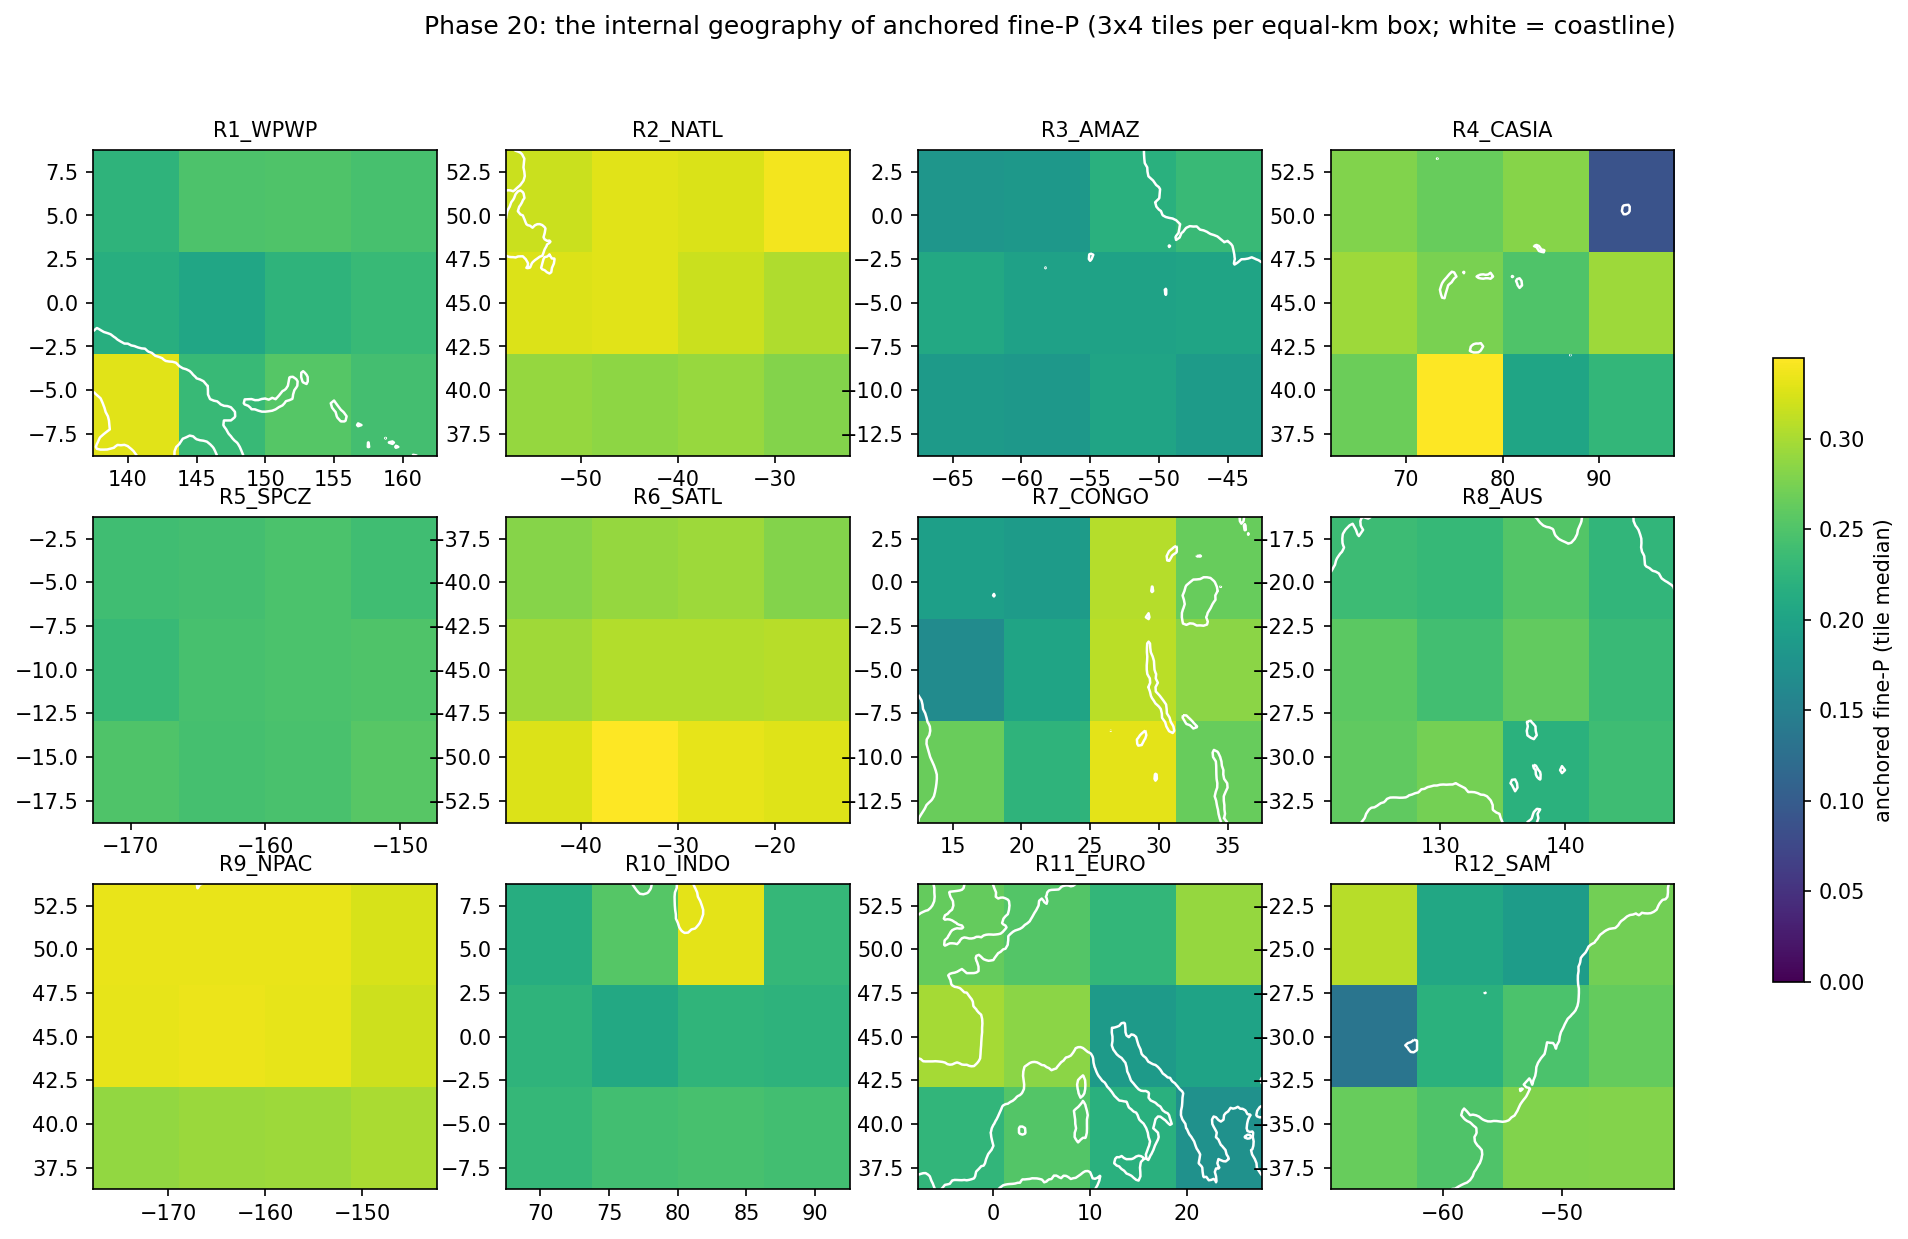
\includegraphics[width=\linewidth]{figures/fig2_tile_maps.png}
\caption{Внутренняя география тонкомасштабного $P$ с суррогатной поправкой (полосы 50--400~км): 12 равновеликих областей $\times$ 12 тайлов, медианы по окнам; белым --- береговая линия. Максимумы приходятся на области внетропических штормовых путей --- североатлантическую (R2), южноатлантическую (R6) и северотихоокеанскую (R9); минимумы --- на ядра глубокой конвекции (запад бассейна Конго, Амазония) и на северо-восточный тайл Центральной Азии.}
\label{fig:tiles}
\end{figure}

\begin{figure}[t]
\centering
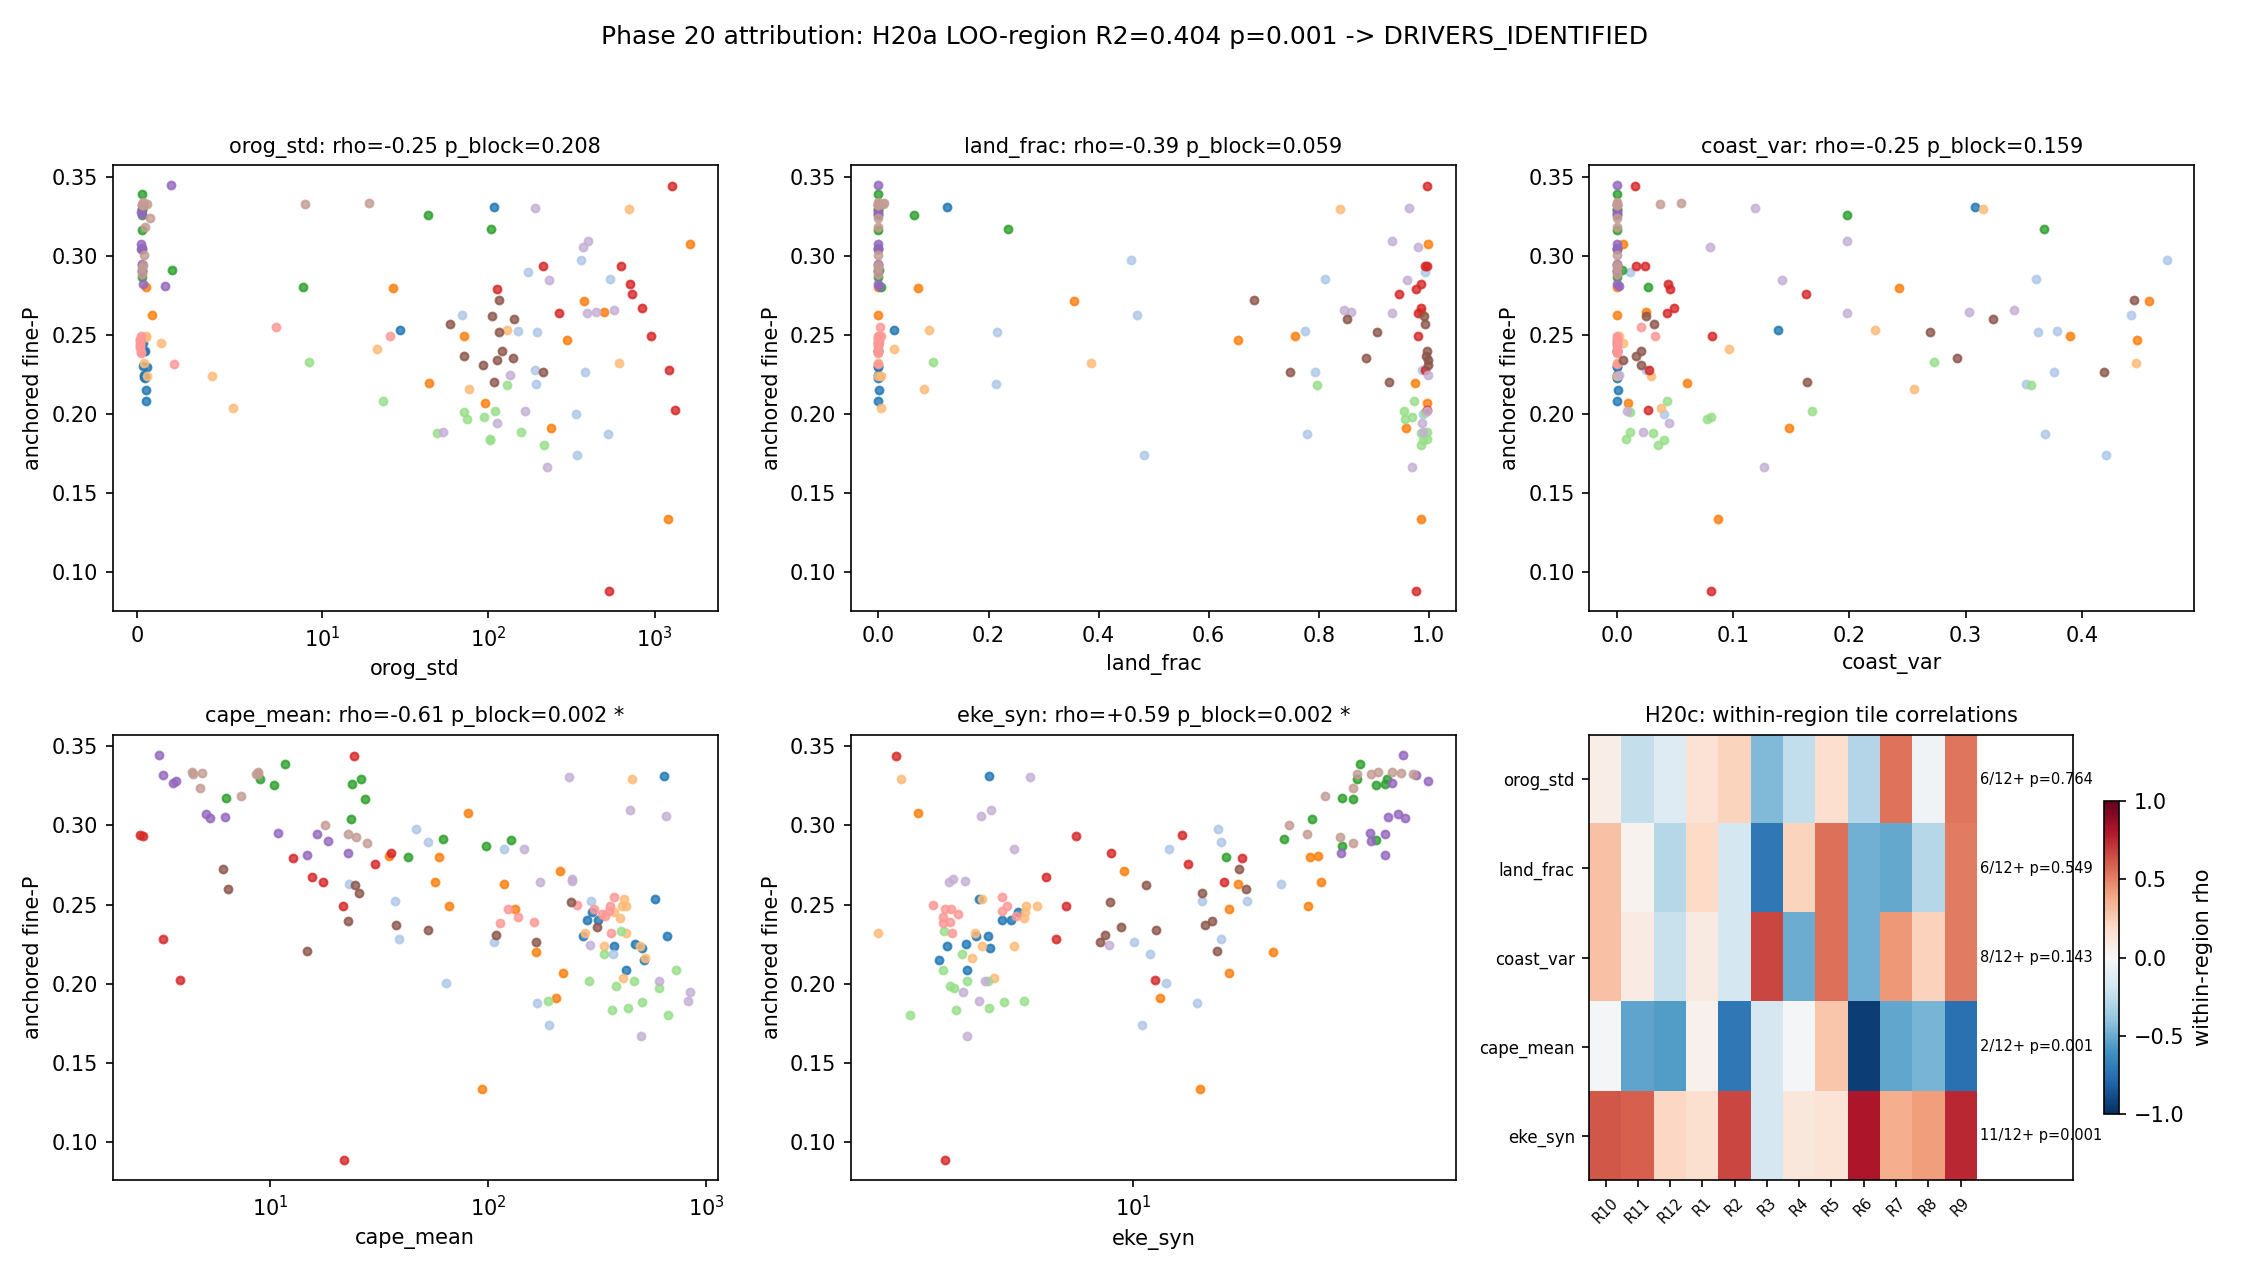
\includegraphics[width=\linewidth]{figures/fig2_attribution.png}
\caption{Часть A, атрибуция тайлового $P$: диаграммы рассеяния по пяти ковариатам с $p$-значениями блочного нуля (цвет --- регион; звёздочкой отмечены значимые связи) и тепловая карта внутрирегиональных корреляций (справа внизу): CAPE отрицательна в 10 из 12 регионов, синоптическая вихревая энергия положительна в 11 из 12.}
\label{fig:attrA}
\end{figure}

\subsection{Атрибуция карты: чем связана её география (часть B)}
\label{sec:armB}

Атрибуция глобальной карты выполнена по восьми заранее заявленным ковариатам с выбыванием целых секторов долготы и нуль-моделью вращения; сводка --- в табл.~\ref{tab:armB}, посезонные карты и кривая пошагового отбора --- на рис.~\ref{fig:seasons}. Карта части~B согласована с картой части~A на 133 общих тайлах ($\rho=0{,}840$). Результат складывается в три утверждения.

\emph{Первое: атрибуция значима, и её значимость незональна.} Восемь ковариат предсказывают карту вне сектора подгонки с $R^2=0{,}536$ ($p=0{,}001$ при 95-м перцентиле нуля 0,455). Поскольку нуль-модель вращения сохраняет всю зональную структуру целиком --- модуль широты инвариантен относительно поворота долготы, --- значимость удостоверяет привязку карты к \emph{конкретному долготному положению} штормовых путей и конвективных очагов. Ни одна широтная закономерность сама по себе такого результата дать не может. Отрицательный контроль чист: индекс листовой поверхности даёт прирост $-0{,}004$ ($p=0{,}832$), скрытого смешения в схеме нет.

\emph{Второе: карта эффективно одномерна.} Пошаговый отбор показывает, что одна ковариата --- синоптическая вихревая энергия --- даёт $R^2=0{,}456$, то есть 85\,\% полного качества предсказания ($k_{80}=1$). География сопряжённости, взятая как задача районирования, упорядочивается практически одной осью, и эта ось --- активность внетропических штормовых путей. Факт эмпирический и от теоретической интерпретации не зависит.

\emph{Третье: связь двухканальна.} Это главный результат части~B, и виден он не в величине $R^2$, а в составе нагрузок (табл.~\ref{tab:loadings}, рис.~\ref{fig:channels}). Контрольная мишень --- наклон пространственного спектра тайла --- предсказывается теми же восемью ковариатами \emph{не хуже} целевой величины ($R^2=0{,}570$ против $0{,}536$). Но наборы ведущих ковариат у двух мишеней практически не пересекаются: сопряжённость нагружают вихревая энергия ($+0{,}66$), модуль широты ($+0{,}66$), градиент ТПО ($+0{,}55$) и CAPE ($-0{,}52$), тогда как спектральный наклон --- расчленённость рельефа ($+0{,}74$), доля суши ($+0{,}67$), средняя высота рельефа ($+0{,}65$) и изрезанность берега ($+0{,}63$). Ведущие ковариаты одной мишени лежат в полосе $\lvert\rho\rvert<0{,}3$ у другой. Двухканальная структура, найденная в части~A внутри регионов, воспроизводится, таким образом, на глобальной сетке: повышение сопряжённости при высокой штормовой активности идёт через ту же дисперсионную структуру, которую видит спектр, а понижение при высокой конвективной неустойчивости лежит сверх спектра.

Разделение по ярусам добавляет к этой картине существенную деталь: один ярус~1 (экзогенные граничные условия) даёт $R^2=0{,}482$ при $p=0{,}002$, а ярус~2 добавляет к этому лишь $+0{,}053$. То есть 90\,\% полного качества предсказания восстанавливается по одним лишь стационарным условиям территории. Следствия для выбора между H1 и H2 разобраны в разд.~\ref{sec:interp}.

\begin{table}[t]
\centering
\caption{Часть B: сводка проверок на глобальной сетке (902 тайла после орографического исключения). LOSO --- выбывание по сектору долготы $60^\circ$; нуль --- вращение долготной сетки ковариат (999 повторов).}
\label{tab:armB}
\small
\begin{tabular}{@{}p{0.46\linewidth}p{0.48\linewidth}@{}}
\toprule
Проверка & Итог\\
\midrule
Согласованность с частью A (133 общих тайла) & $\rho=0{,}840$ (заранее заданный порог 0,7)\\
Атрибуция, выбывание по сектору & $R^2=0{,}536$; $p=0{,}001$ (95-й перцентиль нуля 0,455)\\
Разделение по ярусам & ярус 1 (граничные условия): $R^2=0{,}482$ ($p=0{,}002$); прирост от яруса 2: $+0{,}053$\\
Эффективная размерность & одна вихревая энергия: $R^2=0{,}456$, т.\,е. 85\,\% полного качества; $k_{80}=1$\\
Потолок надёжности карты (внутрисезонное расщепление пополам) & $R^2=0{,}914$; атрибуция объясняет 59\,\% воспроизводимой дисперсии\\
Контрольная мишень: наклон спектра & $R^2=0{,}570$ --- не хуже целевой величины, но с непересекающимся набором ведущих ковариат (рельеф и доля суши вместо вихревой энергии, широты, градиента ТПО и CAPE)\\
Отрицательный контроль (индекс листовой поверхности) & прирост $-0{,}004$; $p=0{,}832$ --- контроль чист\\
Сезонная устойчивость карты & медиана $\lvert$ЯФМ$-$ИАС$\rvert=0{,}016$ (ЯФМ --- январь--март, ИАС --- июль--сентябрь) (90-й перцентиль 0,048)\\
\bottomrule
\end{tabular}
\end{table}

\begin{table}[t]
\centering
\caption{Нагрузки восьми ковариат (ранговая корреляция по 902 тайлам) на две мишени: $P$ с суррогатной поправкой и наклон пространственного спектра тайла. Мишени предсказываются сопоставимо хорошо ($R^2_{\mathrm{LOSO}}=0{,}536$ и $0{,}570$), но ведущими для них оказываются непересекающиеся наборы ковариат --- в этом и состоит двухканальная структура связи. Ярус~2 отмечен звёздочкой.}
\label{tab:loadings}
\small
\begin{tabular}{@{}lcc@{}}
\toprule
Ковариата & $P$ с поправкой & Наклон спектра\\
\midrule
Синоптическая вихревая энергия${}^{*}$ & $+0{,}66$ & $-0{,}12$\\
Модуль широты & $+0{,}66$ & $-0{,}05$\\
Градиент ТПО & $+0{,}55$ & $-0{,}27$\\
Климатология CAPE${}^{*}$ & $-0{,}52$ & $+0{,}22$\\
Доля суши & $-0{,}17$ & $+0{,}67$\\
Орография (станд. отклонение) & $-0{,}14$ & $+0{,}74$\\
Орография (средняя высота) & $-0{,}11$ & $+0{,}65$\\
Контрастность суша--море & $-0{,}05$ & $+0{,}63$\\
\bottomrule
\end{tabular}
\end{table}

\begin{figure}[t]
\centering
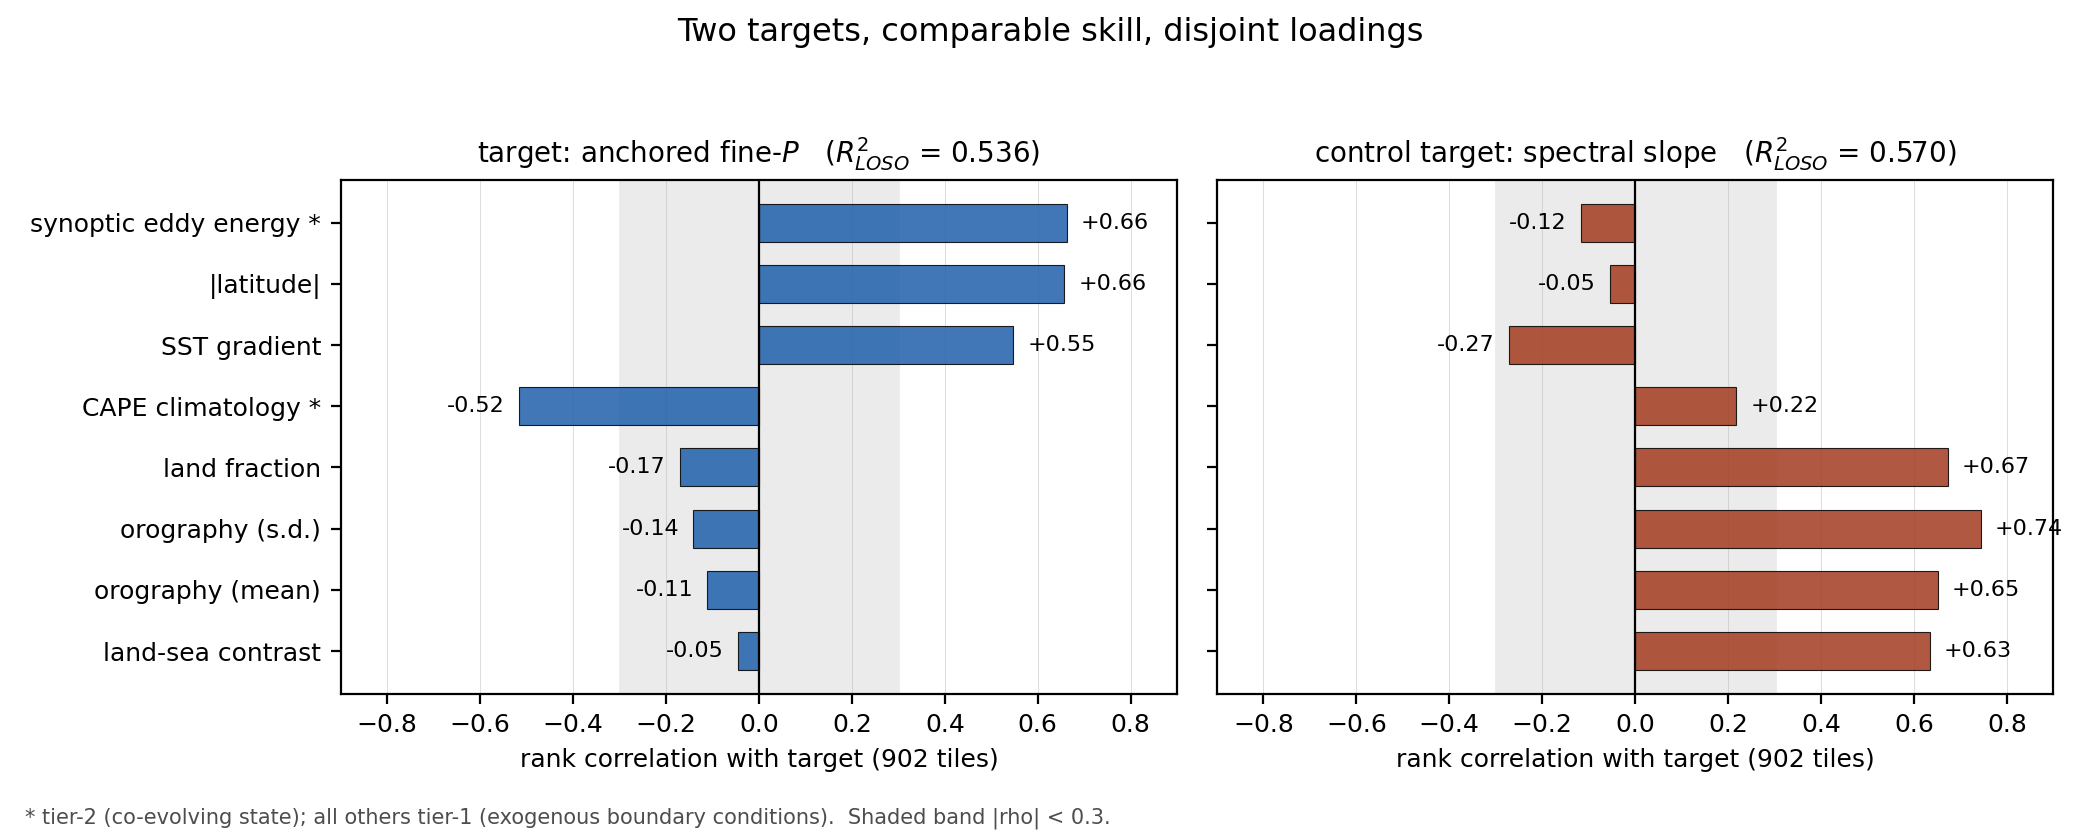
\includegraphics[width=\linewidth]{figures/fig2_channels.png}
\caption{Двухканальная структура связи: нагрузки восьми ковариат на две мишени глобальной тайловой карты --- $P$ с суррогатной поправкой (слева) и наклон пространственного спектра (справа), 902 тайла. Обе мишени предсказываются по одному и тому же набору ковариат сопоставимо хорошо (значения $R^2$ при выбывании сектора долготы --- в заголовках панелей), однако ведущие ковариаты у них разные: серая полоса отмечает диапазон $\lvert\rho\rvert<0{,}3$, и ведущие ковариаты каждой мишени попадают внутрь этой полосы у другой. Звёздочкой помечены характеристики яруса~2 (совместно складывающееся состояние), остальные --- ярус~1 (экзогенные граничные условия).}
\label{fig:channels}
\end{figure}

\begin{figure}[t]
\centering
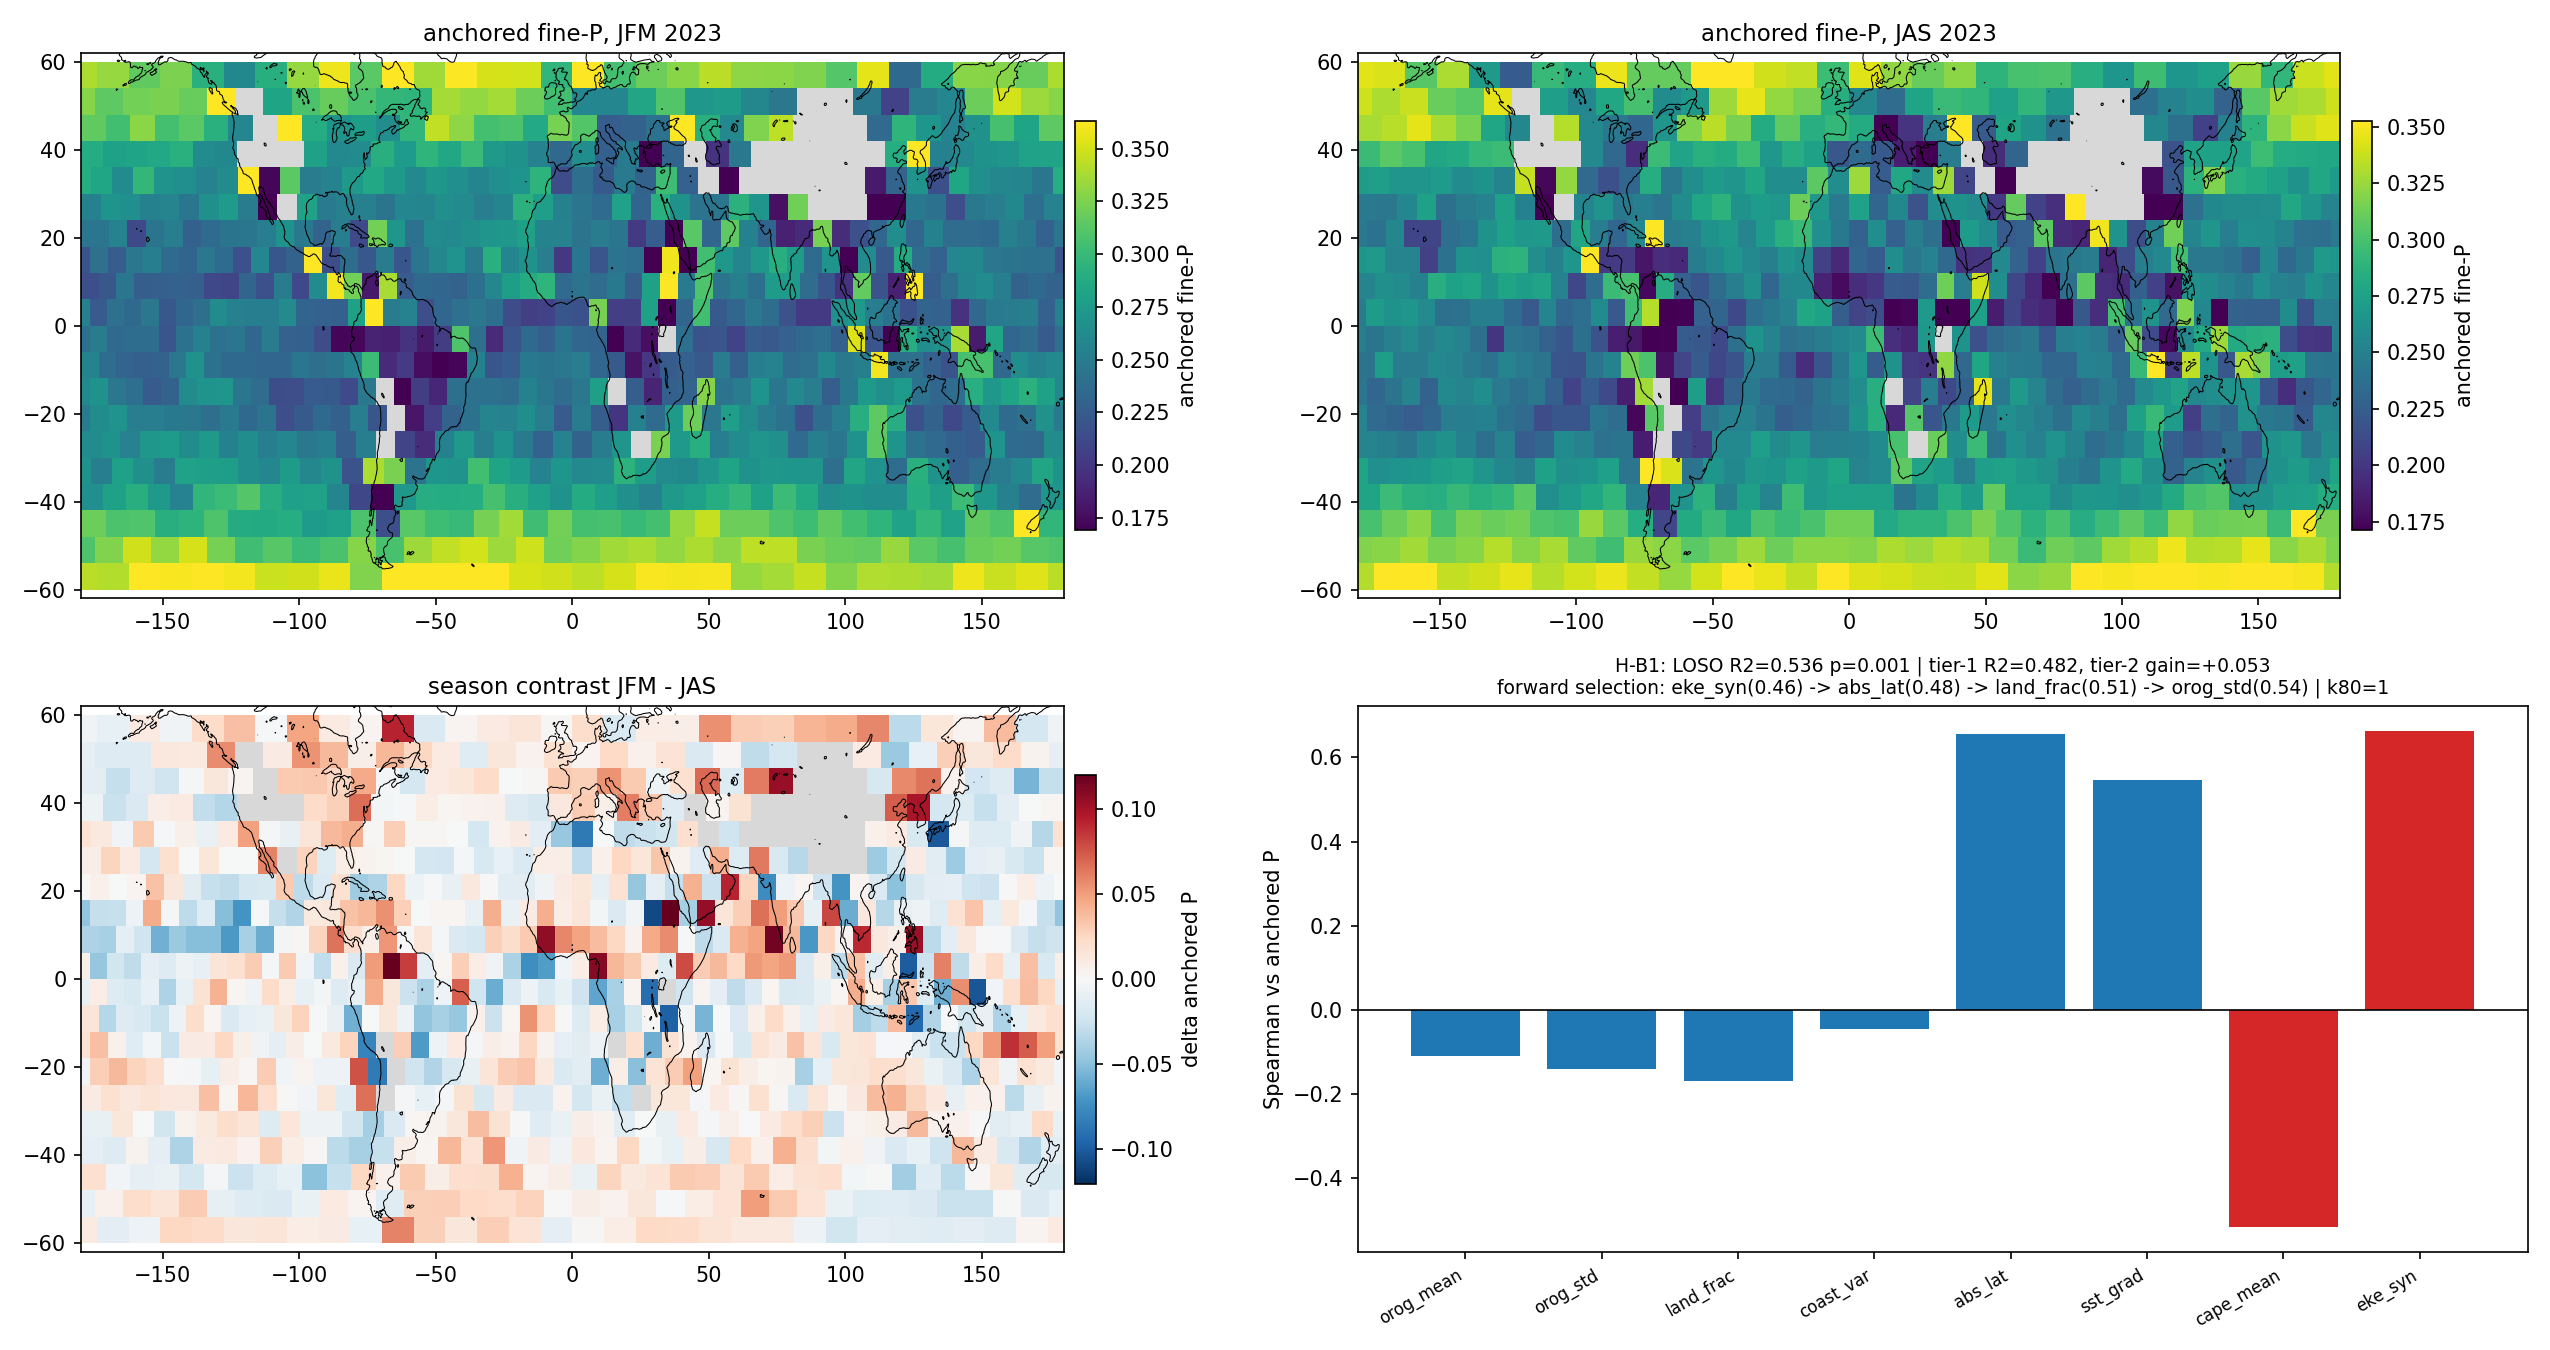
\includegraphics[width=\linewidth]{figures/fig2_seasons_attribution.png}
\caption{Часть B, сезонная структура и атрибуция: карты $P$ (с суррогатной поправкой) по сезонам январь--март и июль--сентябрь 2023~г. (вверху), сезонный контраст (внизу слева; медиана модуля 0,016) и нагрузки восьми ковариат с кривой пошагового отбора (внизу справа): вихревая энергия одна даёт $R^2=0{,}456$ из полных $0{,}536$.}
\label{fig:seasons}
\end{figure}

\subsection{Полнота атрибуции и воспроизводимый остаток}
\label{sec:residual}

Долю карты, которую восемь ковариат объясняют, следует считать не от полной дисперсии, а от той её части, которая вообще воспроизводима. Потолок восстановимости карты, оценённый внутрисезонным расщеплением выборки пополам, составляет $R^2=0{,}914$; межсезонная оценка ($0{,}603$) занижает его, поскольку списывает реальное сезонное изменение карты на счёт шума. Относительно этого потолка заявленные ковариаты объясняют 59\,\% воспроизводимой дисперсии: карта атрибутирована, но далека от насыщения. Добавление четырёх статистик интермиттентности огибающих --- ближайших статистических родственников~$P$; сам параметр интермиттентности восходит к уточнённой гипотезе подобия \cite{Kolmogorov1962} --- поднимает предсказание совместной модели до $R^2=0{,}761$, то есть до 83\,\% воспроизводимой дисперсии. Что этот прирост не является общим выборочным шумом двух блоков, показано отдельно: при вычислении~$P$ и статистик интермиттентности на непересекающихся половинах выборки прирост сохраняется и составляет $+0{,}207$ в среднем по четырём расщеплениям ($p=0{,}001$; без декорреляции он равен $+0{,}261$, то есть доля общего шума --- около одной пятой). Систематическое положение этого блока среди родственных статистик разобрано в третьей статье серии.

Остаток после ковариат и блока интермиттентности --- около 15\,\% воспроизводимой дисперсии --- \emph{не является шумом}. Он воспроизводится между независимыми половинами выборки ($r=0{,}64$ при пороге решающего правила $0{,}30$), не сводится к спектральным признакам ($\lvert\rho\rvert\le0{,}12$ с наклоном и логарифмическими дисперсиями полос) и обнаруживает географически организованный рисунок: отрицательные значения преобладают на муссонных окраинах \cite{RodwellHoskins1996} и наветренных склонах горных систем, положительные --- над очагами глубокой конвекции и высокоширотными окраинами материков. Существование воспроизводимого остатка --- самостоятельный результат; его географический рисунок здесь только описан, но не атрибутирован.

Попытка атрибуции остатка предпринята и завершилась отрицательным вердиктом. Простейший орографический кандидат --- расстояние тайла до ближайшего рельефа выше 1200~м --- прироста не даёт ($\Delta R^2\approx0$; апостериорная проверка). Блок из четырёх гидроклиматических кандидатов (годовая амплитуда осадков, конвективная доля осадков, вертикальный сдвиг ветра 850--500~гПа, влагозапас), проверенный по отдельному зафиксированному до вычислений протоколу (\texttt{PROTOCOL\_PHASE25} в репозитории), заранее заданного порога прироста не проходит ($+0{,}024$ при пороге $+0{,}03$): три кандидата уже поглощены базовым набором через конвективно-влажностный канал. Единственная содержательная находка --- вертикальный сдвиг ветра: лишь он значимо связан с воспроизводимым остатком ($\rho=-0{,}38$, $p=0{,}001$ при вращательном нуле), связь не опосредована спектром (прирост к контрольной мишени $+0{,}008$), и он один несёт почти весь прирост блока ($+0{,}027$). Кандидат содержателен --- вертикальный сдвиг служит классическим управляющим параметром пространственной организации конвекции \cite{RotunnoKlempWeisman1988,Wing2017}, --- но по действующим правилам программы вердикт проверки отрицательный, и утверждение об атрибуции остатка не делается. Сдвиг ветра остаётся единственным именованным кандидатом для отдельной будущей проверки; в остальном идентификация источников остатка в настоящей серии не выполняется.

\subsection{Природа карты: физика атмосферы или артефакт наблюдений}
\label{sec:model}

Сопоставление двух реанализов не отделяет свойство атмосферы от свойства наблюдательной сети: обе системы усваивают в основном одни и те же наблюдения \cite{Hersbach2020,Gelaro2017}; решающая проверка --- расчёт, не усваивающий наблюдений. Использован эксперимент \texttt{highresSST-present} проекта HighResMIP \cite{Haarsma2016} по модели ECMWF-IFS-HR \cite{Roberts2018}: расчёт типа AMIP --- атмосфера при заданной наблюдаемой температуре поверхности океана \cite{Gates1992}; глобальные поля 2014~г., разрешение $0{,}5^\circ$, без усвоения атмосферных наблюдений.

На 902 тайлах, согласованных по разрешению, ранговая корреляция эталонной пары <<ERA5 при $0{,}25^\circ$ --- ERA5 при $0{,}5^\circ$>> (одна и та же атмосфера, цена огрубления метода) составляет $0{,}897$ --- это разрешающий предел сопоставления. Карта свободного расчёта воспроизводит карту ERA5 с $\rho=0{,}869$, то есть \emph{97\,\% достижимого согласия} (здесь и далее --- отношение ранговых корреляций, а не доля объяснённой дисперсии), при том что расчёт относится к другому году (2014 против 2023) и не видел ни одного атмосферного наблюдения (рис.~\ref{fig:round2}, слева). Нагрузки ковариат на модельную карту повторяют реанализные: вихревая энергия $+0{,}68$; модуль широты $+0{,}70$; градиент ТПО $+0{,}51$; CAPE $-0{,}50$; рельеф $\approx0$. Глобальная карта сопряжённости --- свойство физики атмосферы при заданных граничных условиях, а не артефакт наблюдательной сети или системы усвоения.

Смысл этой пары чисел стоит проговорить прямо: 0,897 --- не идеал, а потолок, задаваемый самим огрублением разрешения, поэтому 0,869 означает не <<87\,\% совпадения>>, а почти всё, что при таком сопоставлении в принципе достижимо. Следствие гипотезы H3 не выполнено, и H3 отвергается.

Во избежание путаницы при совместном чтении с первой статьёй серии: там для сопоставления со свободным расчётом приводится величина $\rho=0{,}71$ при пределе $0{,}93$ --- она относится к \emph{региональной} выборке по 39 областям (2017--2024~гг.). Приведённая здесь пара $0{,}869/0{,}897$ относится к \emph{глобальной мозаичной} выборке (902 тайла, $0{,}5^\circ$, 2014 против 2023~гг.); эти величины получены на разных выборках и не взаимозаменяемы.

\begin{figure}[t]
\centering
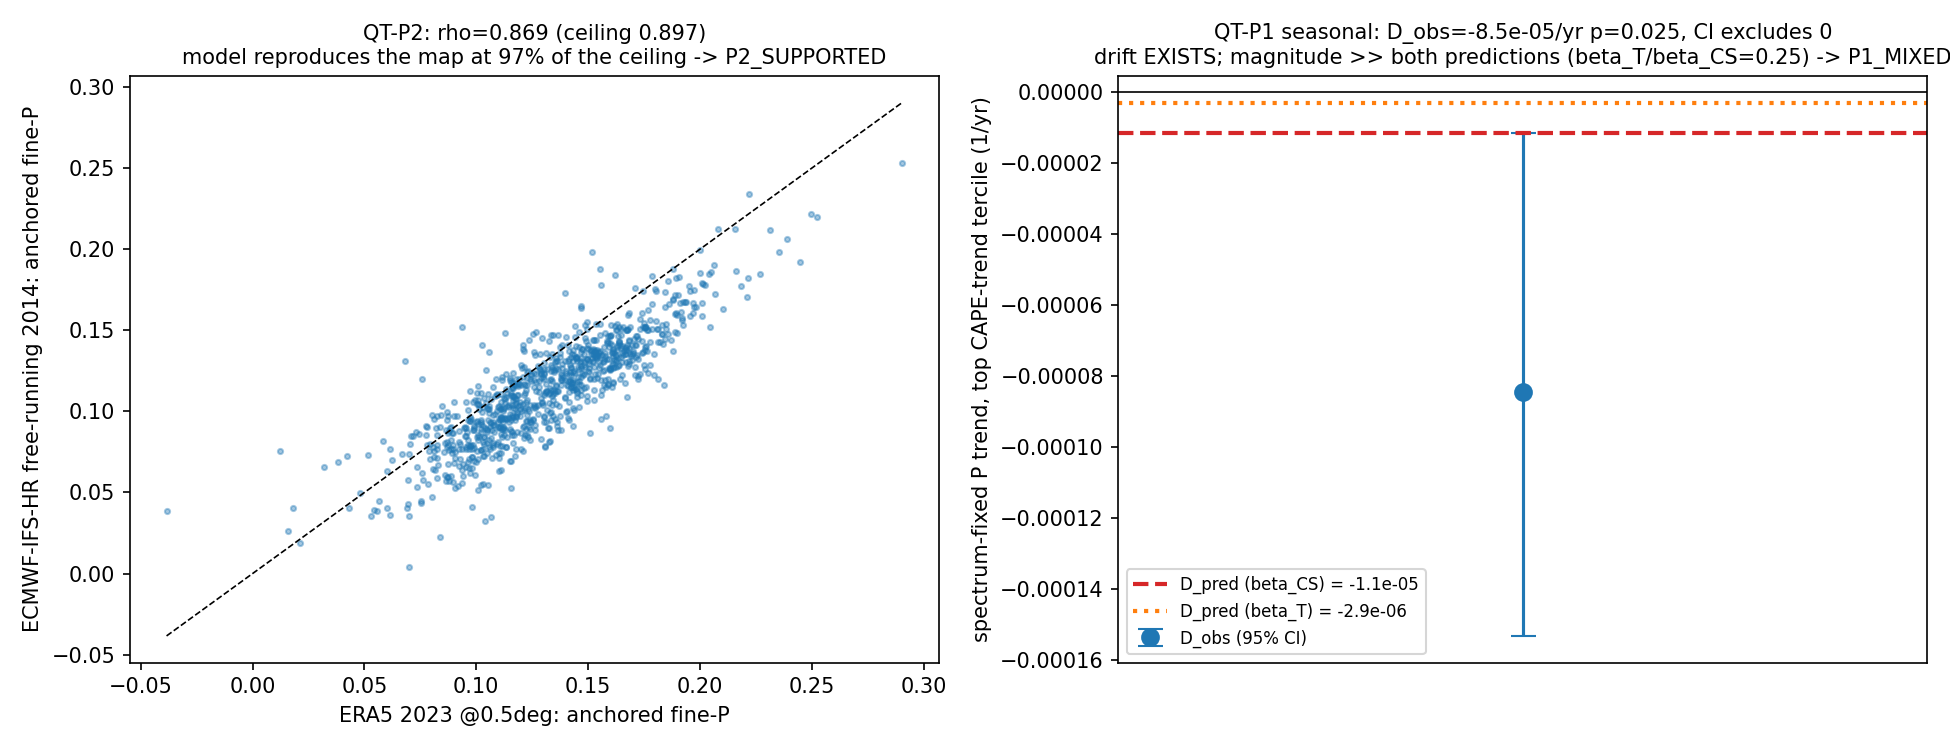
\includegraphics[width=\linewidth]{figures/fig2_qt_round2.png}
\caption{Слева: тайловая карта $P$ (с суррогатной поправкой) свободного расчёта ECMWF-IFS-HR (2014~г., без усвоения наблюдений) против карты ERA5 (2023~г.) на 902 согласованных по разрешению тайлах: $\rho=0{,}869$ при разрешающем пределе $0{,}897$; пунктир --- линия равенства. Справа: тренд спектрально-фиксированного $P$ в тайлах верхней терцили тренда CAPE (точка --- оценка, отрезок --- 95-\%-й доверительный интервал кластерного бутстрэпа) в сравнении с двумя калибровочными предсказаниями (штриховые линии); к разд.~\ref{sec:static}.}
\label{fig:round2}
\end{figure}

\subsection{Дополнительная проверка: тропический избыток межгодовой изменчивости}
\label{sec:ipo}

На длинной записи (1979--2024~гг.) двенадцать областей программы демонстрируют высокую устойчивость межгодовых значений инварианта, за одним исключением: три очага глубокой конвекции --- тёплый бассейн запада тропической части Тихого океана, Амазония и Южно-Тихоокеанская зона конвергенции --- несут избыток межгодовой дисперсии карт активности ($F=1{,}75$; $2{,}24$ и $2{,}07$ соответственно, против $0{,}70$--$1{,}35$ у остальных девяти областей), устойчивый к смене единицы выборки. Связь этого избытка с ЭНСО (индекс ONI \cite{Trenberth1997}) исключена прямым тестом при тридцатикратном превышении статистической мощности относительно первоначальной восьмилетней проверки (2017--2024~гг.).

Для атрибуции избытка заранее --- до обращения к данным --- был назван список из четырёх климатических индексов (PDO \cite{Newman2016}, AMO, DMI, IPO-TPI \cite{Henley2015}); статистика теста --- максимум ранговой корреляции по восьми комбинациям <<индекс $\times$ сглаживание>> с совместным нулём циклического сдвига по времени, штрафующим за множественность выбора. Результаты --- в табл.~\ref{tab:ipo} и на рис.~\ref{fig:ipo}.

\begin{table}[t]
\centering
\caption{Атрибуция тропического избытка межгодовой изменчивости по заранее названным индексам (максимум-статистика по 8 комбинациям <<индекс $\times$ сглаживание>>, совместный нуль циклического сдвига).}
\label{tab:ipo}
\small
\begin{tabular}{@{}lcccc@{}}
\toprule
Регион & $T=\max\lvert\rho\rvert$ & Лучший индекс & $p$ & Значимо\\
\midrule
Тёплый бассейн запада тропической Пацифики & 0,311 & PDO (5-летнее сглаж.) & 0,155 & нет\\
Амазония & 0,453 & IPO-TPI & 0,001 & да\\
Южно-Тихоокеанская зона конвергенции & 0,602 & IPO-TPI & 0,001 & да\\
\bottomrule
\end{tabular}
\end{table}

Совпадение ведущего индекса в двух из трёх регионов активирует заранее зафиксированное правило согласованности: тропический избыток --- проявление \emph{декадной} моды, Междекадного тихоокеанского колебания (IPO) \cite{Power1999,Henley2015}, а не межгодового ЭНСО-режима. Третий регион (тёплый бассейн запада тропической части Тихого океана, самый слабый избыток) остаётся неатрибутированным.

\begin{figure}[t]
\centering
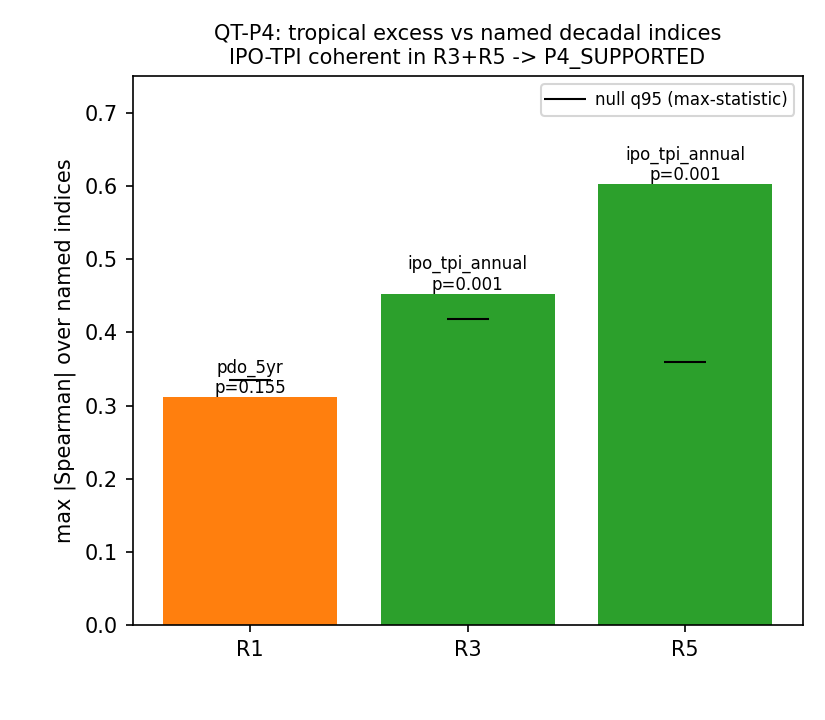
\includegraphics[width=0.6\linewidth]{figures/fig2_ipo.png}
\caption{Максимум-статистика связи межгодовой дисперсии карт активности с заранее названными климатическими индексами для трёх очагов тропического избытка межгодовой изменчивости; горизонтальные отрезки --- 95-е перцентили совместного нуля циклического сдвига. В Амазонии (R3) и Южно-Тихоокеанской зоне конвергенции (R5) значим один и тот же индекс --- IPO-TPI.}
\label{fig:ipo}
\end{figure}

\subsection{Проверка гипотезы статичности}
\label{sec:static}

Если~$P$ --- статичная характеристика сложившегося режима, он по определению не должен опережать перестройку этого режима и не должен превосходить по чувствительности стандартные показатели среднего поля. Это следствие проверено прямо; итоги сведены в табл.~\ref{tab:static}.

\emph{Реакция на известную перестройку режима.} Единственный крупный документированный сдвиг внутри записи --- переход Междекадного тихоокеанского колебания 1998/99~гг. На 72 парах <<тайл--сезон>> трёх тропических регионов сопоставлены статистики перехода четырёх показателей. Доля случаев, в которых~$P$ реагирует на переход раньше или резче конкурента, составила: против CAPE --- 25\,\%, против синоптической вихревой энергии --- 47\,\%, против наклона спектра --- 42\,\% при пороге опережающего поведения 60\,\%. По медианному отношению <<сигнал/шум>> многолетнего тренда на 288 парах <<тайл--сезон>> $P$ занимает последнее место из четырёх: CAPE --- 2,39; наклон спектра --- 1,03; вихревая энергия --- 0,85; $P$ --- 0,67. Ни одно из трёх парных сравнений не свидетельствует в пользу более высокой чувствительности~$P$ ($p=1{,}000$ в каждом; проверялась односторонняя гипотеза о превосходстве~$P$ над конкурентом). Для инварианта, по построению не несущего собственной динамики, это ожидаемое поведение, прямо подтверждающее исходную гипотезу: величина регистрирует архитектуру уже сложившегося режима и не выступает опережающим индикатором его перестройки.

\emph{Отдельный и открытый вопрос --- многодесятилетняя устойчивость самого инварианта.} На сезонной выборке (288 пар <<тайл--сезон>>, не менее 30 лет каждая) в тайлах верхней терцили тренда CAPE обнаружен слабый отрицательный тренд спектрально-фиксированного~$P$: $-8{,}5\cdot10^{-5}$~год$^{-1}$, $p=0{,}025$, доверительный интервал кластерного бутстрэпа исключает ноль (рис.~\ref{fig:round2}, справа). Величина тренда примерно в семь раз превышает кросс-секционную калибровку по пространственному контрасту CAPE и почти в тридцать раз --- калибровку по межгодовой ковариации: отклик, если он реален, зависит от временного масштаба воздействия. Однако единственный доступный свободный расчёт с переходным форсингом воспроизводит тренд того же знака лишь на $\sim$27\,\% величины и статистически неотличим от нуля ($p=0{,}221$). Это вопрос иного типа, чем предсказательная сила: речь о стабильности самих условий, задающих инвариант, на масштабе десятилетий. На сегодняшних данных он не решён: факт тренда установлен только внутри ERA5 --- записи, охватывающей крупные смены наблюдательной системы, вследствие чего многолетние тренды в реанализах требуют особой осторожности \cite{Bengtsson2004}, --- и модельное подтверждение его физической природы отсутствует. Мы оставляем статус вопроса явно открытым.

\begin{table}[t]
\centering
\caption{Сводка проверки гипотезы статичности инварианта.}
\label{tab:static}
\small
\begin{tabular}{@{}p{0.47\linewidth}p{0.47\linewidth}@{}}
\toprule
Проверка & Итог\\
\midrule
Опережает ли $P$ стандартные показатели на переходе 1998/99~гг. (порог 60\,\%) & нет: опережение против CAPE в 25\,\% случаев, против вихревой энергии в 47\,\%, против наклона спектра в 42\,\% --- согласуется с гипотезой статичности\\
Чувствительность к многолетнему тренду (медианное сигнал/шум, 288 пар <<тайл--сезон>>) & $P$ --- последний из четырёх показателей: 0,67 против 2,39 (CAPE), 1,03 (наклон спектра), 0,85 (вихревая энергия); гипотеза о превосходстве $P$ отвергается во всех трёх парных сравнениях ($p=1{,}000$)\\
Тренд спектрально-фиксированного $P$ в тайлах наибольшего тренда CAPE (ERA5) & $-8{,}5\cdot10^{-5}$~год$^{-1}$, $p=0{,}025$, доверительный интервал исключает ноль\\
Тот же тренд в свободном расчёте с переходным форсингом & тот же знак при $\sim$27\,\% величины, $p=0{,}221$ --- физичность тренда не подтверждена, вопрос открыт\\
\bottomrule
\end{tabular}
\end{table}

\section{Интерпретация: ответ на исходные гипотезы}
\label{sec:interp}

Соберём ответы. \emph{H3 отвергнута}: карта воспроизводится свободным расчётом, не усваивающим атмосферных наблюдений, на 97\,\% достижимого согласия, и потому не может быть артефактом наблюдательной сети. \emph{H1 и H2 обе подтверждены --- и именно это составляет результат.} Наибольшую индивидуальную нагрузку несёт характеристика яруса~2 (вихревая активность, $k_{80}=1$), и связь сохраняется внутри регионов, где экзогенные условия почти постоянны, --- следствие H2 выполнено. Одновременно один ярус~1 восстанавливает 90\,\% полного качества предсказания --- следствие H1 выполнено тоже. Противоречия здесь нет: климатическое положение штормовых путей и очагов глубокой конвекции само есть следствие распределения материков, океанов и горных систем, поэтому два яруса читают, по существу, одну и ту же карту с разных сторон. Подчеркнём, что данные \emph{не} позволяют утверждать, будто рельеф и океан действуют исключительно опосредованно, через режимы: при 90\,\% качества у одного яруса~1 такое утверждение было бы сильнее данных.

Отсюда итоговая формулировка, объединяющая обе подтверждённые гипотезы: \emph{географическая дифференциация сопряжённости уровней структурирована через размещение атмосферных циркуляционных режимов в географическом пространстве, а размещение самих режимов задано экзогенной конфигурацией территории}. В цепочке <<конфигурация $\to$ организация процессов $\to$ сопряжённость>> настоящей работой установлены оба крайних звена и их согласованность, но не механизм перехода между ними.

Разделение ковариат на ярусы задаёт и допустимый язык итоговой интерпретации. Для яруса~1 --- орографии, конфигурации суши и океана, широты, градиента температуры поверхности океана --- направленная формулировка <<граничные условия формируют географию сопряжённости>> корректна: эти поля экзогенны по отношению к циркуляции на любых рассматриваемых временных масштабах. Для яруса~2 --- синоптической вихревой активности и конвективного режима --- направленный язык не используется: их связь с~$P$ достигает максимума при нулевом временном сдвиге, без опережения в какую-либо сторону, и корректная формулировка --- \emph{совместное формирование}: сопряжённость уровней, штормовая активность и конвективный режим суть согласованные проявления одной установившейся организации циркуляции, а не звенья причинной цепи друг для друга.

Профиль при этом естественно читать как наблюдаемую проекцию установившейся статистики быстрой динамики циркуляции при фиксированном на масштабе наблюдения поле внешних условий. Развёртывание этой интерпретации, её следствия и границы применимости --- предмет третьей статьи серии; проверка самих механизмов, связывающих циркуляционный режим с устройством межуровневых связей, составляет задачу отдельного исследования, тогда как статистическая связь и её канальное разделение установлены здесь.

\section{Обсуждение и ограничения}
\label{sec:limitations}

Совокупность результатов складывается в определённый статус величины: география сопряжённости уровней --- не случайный рисунок и не артефакт наблюдательной системы, а физически атрибутируемая, эффективно одномерная и воспроизводимая карта, читаемая на языке известных организаторов циркуляции.

Отдельно оценим вес двухканального результата (разд.~\ref{sec:armB}), поскольку именно он, а не величина $R^2$, обосновывает самостоятельность предлагаемой характеристики. Спектр поля скорости --- давно описанная и в общих чертах универсальная характеристика атмосферной турбулентности \cite{NastromGage1985,Lovejoy2011}, и его пространственная изменчивость управляется, как показано выше, свойствами подстилающей поверхности. Если бы география~$P$ читалась тем же набором условий, величина была бы лишь иным способом измерить спектр. Наблюдается противоположное: при сопоставимом качестве предсказания у двух мишеней непересекающиеся ведущие ковариаты. Сопряжённость уровней, следовательно, несёт собственную, не сводимую к спектру географическую информацию --- и в этом качестве может служить самостоятельной координатой районирования.

Пять ограничений заслуживают явной фиксации.

Во-первых, тонкие полосы 50--400~км частично или полностью лежат ниже эффективного разрешения реанализа (разд.~\ref{sec:data}); аргументы разд.~\ref{sec:data} показывают, что карта не является артефактом одного вычислительного тракта, но величина остаётся определённой операционально --- на выходе систем класса реанализа и глобальной модели ($0{,}25$--$0{,}5^\circ$); её перенос на наблюдения километрового разрешения --- открытый вопрос.

Во-вторых, глобальная карта построена по одному году (2023) и двум сезонам. Смягчающие обстоятельства --- сезонная устойчивость карты (медиана контраста 0,016), согласованность с частью~A, охватывающей окна 2021--2024~гг., и воспроизведение карты модельным расчётом 2014~г.; многолетняя глобальная карта остаётся задачей отдельной работы.

В-третьих, проверка природы карты опирается на один свободный расчёт одной модели; желательное усиление --- ансамбль реализаций и модель с иным динамическим ядром.

В-четвёртых, синоптическая вихревая энергия вычисляется из того же поля ветра, что и сам профиль: это два разных функционала одних и тех же данных, и часть их связи может быть завышена общим источником. Верхнюю границу возможной инфляции связи даёт атрибуция только по независимым полям яруса~1: $R^2=0{,}482$ из полных $0{,}536$.

В-пятых, многолетний тренд спектрально-фиксированного профиля установлен только внутри ERA5 --- записи, охватывающей крупные смены наблюдательной системы \cite{Bengtsson2004}, --- и не подтверждён свободным расчётом (разд.~\ref{sec:static}); его статус остаётся открытым.

\section{Выводы}
\label{sec:conclusion}

1.~Географическая дифференциация сопряжённости иерархических уровней циркуляции статистически атрибутируется внешним условиям на двух независимых выборках со согласованными знаками и величинами ($R^2=0{,}404$ на 144 тайлах при выбывании региона и $R^2=0{,}536$ на 902 тайлах при выбывании сектора долготы, $p=0{,}001$). Переход от 39 региональных областей к мозаичной карте решает проблему малой выборки, обесценившую первую попытку атрибуции: половина географии сопряжённости лежит ниже регионального уровня.

2.~Карта --- свойство физики атмосферы, а не наблюдательной системы: свободный модельный расчёт без усвоения наблюдений воспроизводит её на 97\,\% достижимого согласия ($\rho=0{,}869$ при разрешающем пределе $0{,}897$). Гипотеза об артефакте отвергнута.

3.~Связь двухканальна. Штормовая активность сопровождается повышением сопряжённости через ту же дисперсионную структуру, которую отражает спектр; конвективная неустойчивость --- её понижением сверх спектра. Довод не в величине $R^2$, а в составе нагрузок: контрольная мишень (наклон спектра) предсказывается теми же ковариатами не хуже ($0{,}570$ против $0{,}536$), но ведущими для неё оказываются другие ковариаты. Работа устанавливает атрибуцию, а не механизм.

4.~Глобальная карта эффективно одномерна: одна синоптическая вихревая активность даёт 85\,\% полного качества предсказания. При этом она не сводится к широтной зональности --- около половины её дисперсии незональна, и значимость атрибуции удостоверена нуль-моделью, сохраняющей всю зональную структуру.

5.~Экзогенные граничные условия сами по себе дают 90\,\% полного качества предсказания. Экзогенная и циркуляционная гипотезы подтверждаются обе, и это не противоречие: размещение режимов задано конфигурацией материков, океанов и горных систем.

6.~Атрибуция не насыщена. При потолке надёжности карты $R^2=0{,}914$ заявленные ковариаты объясняют 59\,\% воспроизводимой дисперсии, с добавлением статистик интермиттентности --- 83\,\%. Остаток около 15\,\% воспроизводим, не сводится к спектру и географически организован; из проверенных кандидатов значимую связь с ним показал только вертикальный сдвиг ветра, но заранее заданного порога блок не прошёл, и утверждение об атрибуции остатка не делается. Биологический отрицательный контроль чист.

7.~Тропический избыток межгодовой изменчивости в двух из трёх очагов глубокой конвекции статистически связан с Междекадным тихоокеанским колебанием (IPO-TPI, $p=0{,}001$ в обоих регионах при совместном нуле с поправкой на множественность); связь с ЭНСО исключена при тридцатикратном превышении мощности.

8.~Гипотеза статичности подтверждена прямой проверкой: на перестройке циркуляции 1998/99~гг. величина не опережает и не превосходит по чувствительности стандартные показатели режима. Вопрос о медленном многодесятилетнем дрейфе самих условий остаётся открытым: тренд обнаружен только внутри ERA5 и не подтверждён свободным расчётом. Итоговый статус величины, складывающийся из первой статьи серии и настоящей работы, --- воспроизводимая, физически атрибутируемая, глобально картируемая макропеременная сложившихся условий циркуляции; её более широкая теоретическая интерпретация составляет предмет завершающей статьи серии.

\paragraph{Финансирование.} Исследование выполнено без внешнего финансирования.

\paragraph{Конфликт интересов.} Автор заявляет об отсутствии конфликта интересов.

\paragraph{Доступность данных и кода.} Исходные данные --- открыто доступные продукты сторонних поставщиков и в репозитории автора не дублируются: поля ERA5 доступны через Climate Data Store (Copernicus Climate Change Service), модельные расчёты HighResMIP --- через Earth System Grid Federation, ряды климатических индексов --- через NOAA PSL; доступ к CDS требует бесплатной учётной записи. Код анализа, скрипты получения данных, зафиксированные до вычислений протоколы обеих частей, журнал отступлений и производные табличные результаты, достаточные для воспроизведения всех рисунков и статистических проверок работы, открыты в репозитории \url{https://github.com/Theclimateguy/Shroedinger} (версия v6.2; постоянный архив версий --- Zenodo, DOI 10.5281/zenodo.19565769). Маршрут воспроизведения статьи --- от получения данных до каждой таблицы и рисунка --- описан в файле \texttt{reproducibility/article2\_README.md} и автоматизирован скриптом \texttt{reproducibility/reproduce\_article2.py}; там же приведены контрольные суммы ожидаемых артефактов. Описательные величины, не входившие в зафиксированные тесты (разложения дисперсии обеих карт и апостериорная проверка на отложенных бассейнах Конго и Амазонии), пересчитываются скриптом \texttt{clean\_experiments/}\allowbreak\texttt{verify\_article2\_}\allowbreak\texttt{descriptives.py}.

\printbibliography[title={Список литературы}]

\end{document}
